\chapter{Design}

Figure \ref{fig:isys} shows the device developed in this thesis. The following sections describe the design of the sensor system and all components involved.

\begin{figure}[H]
	\begin{center}
		\begin{tikzpicture}
			\node[,inner sep=0] at (0,0) {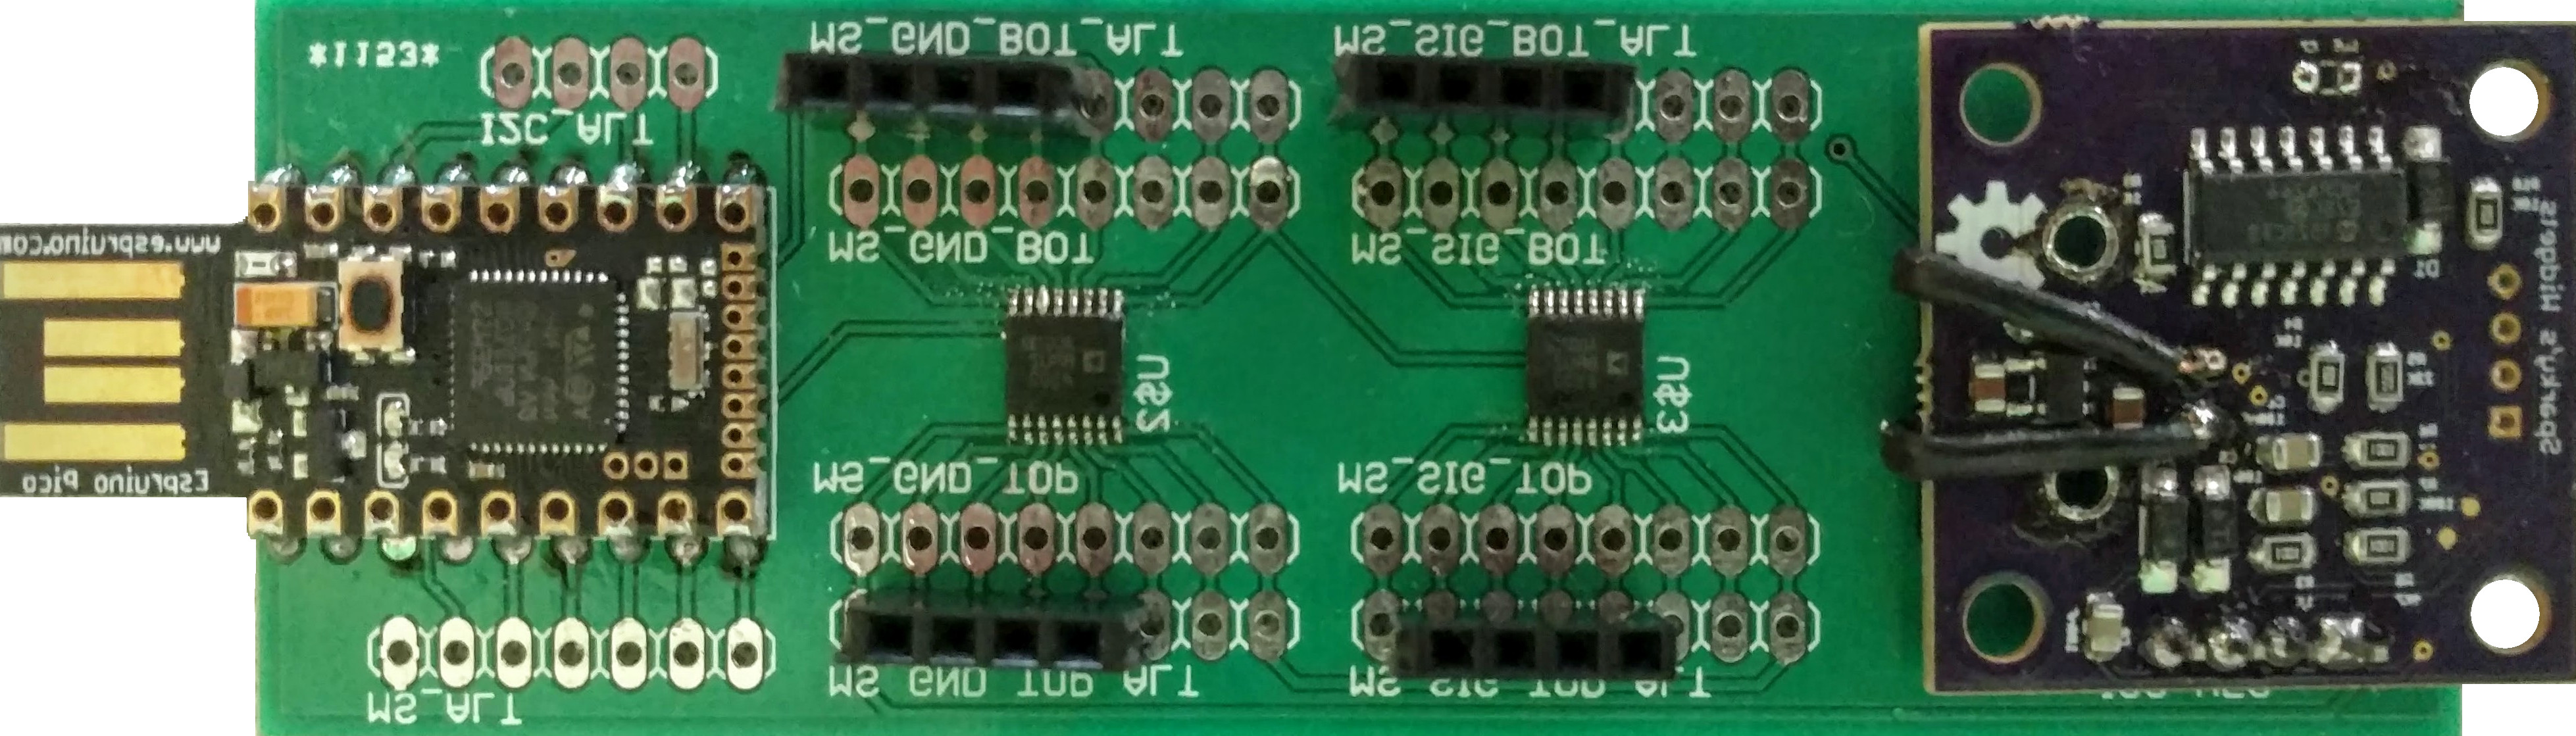
\includegraphics[width=0.5\textwidth]{images/cb.jpg}};
			\node[inner sep=0] at (0,-3) {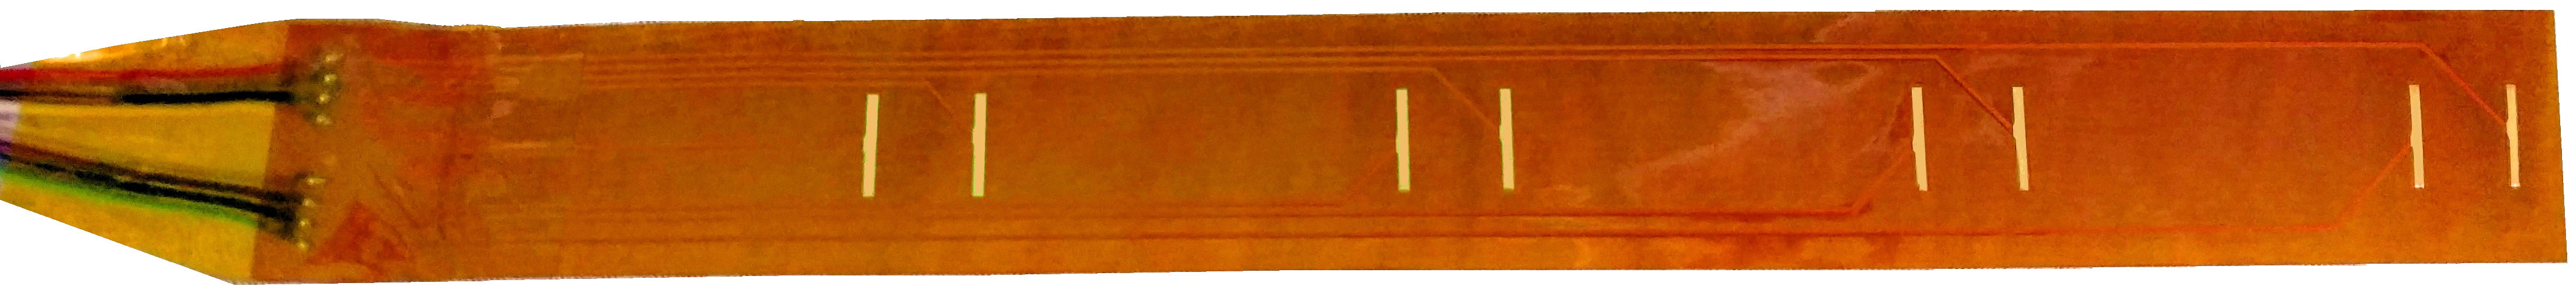
\includegraphics[width=\textwidth]{images/fpcbp.jpg}};
			
			\draw[red,ultra thick,rounded corners] (-4,-0.75) rectangle (-1.5,0.75);
			
			\draw[red!40!yellow,ultra thick,rounded corners] (-1,-0.35) rectangle (-0.25,0.35);
			\draw[red!40!yellow,ultra thick,rounded corners] (0.55,-0.35) rectangle (1.3,0.35);
			
			\draw[red!25!yellow,ultra thick,rounded corners] (-1.45,-1) rectangle (-0.3,-0.6);
			\draw[red!25!yellow,ultra thick,rounded corners] (0.3,-1.05) rectangle (1.3,-0.65);
			\draw[red!25!yellow,ultra thick,rounded corners] (-1.54,1.05) rectangle (-0.44,0.65);
			\draw[red!25!yellow,ultra thick,rounded corners] (0.15,1.05) rectangle (1.15,0.65);
			
			\draw[blue,ultra thick,rounded corners] (1.8,-1.2) rectangle (4,1.2);
			\draw[green,ultra thick,rounded corners] (-8,-4) rectangle (8,-2);
			\draw[blue!50!white,ultra thick,rounded corners] (-2.75,-3.5) rectangle (-1.65,-2.5);
		\end{tikzpicture}
		\caption[The developed sensor system]{The developed sensor system - The microcontroller and USB connection (\drawline[red,ultra thick]) control all parts and connect to the host PC. The matrix switches (\drawline[red!40!yellow,ultra thick]) connect the MinieC (\drawline[blue,ultra thick]) to the sensor strip (\drawline[green,ultra thick]) containing the sensors (\drawline[blue!50!white,ultra thick]) via the connectors (\drawline[red!25!yellow,ultra thick]).}
		\label{fig:isys}
	\end{center}
\end{figure}

\section{System Design} \label{sd}

The system as shown in Figure \ref{fig:sys} is designed as follows:\\
On the user-facing side is a personal computer (PC). This PC runs software that visualizes a live data stream and provides a control interface for the sensor system. It is connected via USB to a microcontroller. This microcontroller controls the MinieC interface via the Inter-Integrated Circuit (I2C) communication protocol, reads the measurement data from it and sends it to the PC. It also controls the matrix switches via the Serial Peripheral Interface Bus (SPI). The MinieC Interface provides the signal (SIG) and ground (GND) between which the resistance is measured. Both lines are connected to one matrix switch each. These matrix switches are able to connect one input to 8 different outputs. On each of those outputs, one electrode is connected. The matrix switches can thereby connect the MinieC interface to one of 8 electrode pairs at a time.

\begin{figure}
	\begin{center}
\begin{tikzpicture}
	\fill [fill=yellow, opacity=0.25] (-5.5,4) rectangle (5,7);
	\fill [fill=green, opacity=0.25] (-5.5,-3.5) rectangle (5,4);
	\fill [fill=blue, opacity=0.25] (5,-3.5) rectangle (10,2);
	\begin{pgfonlayer}{nodelayer}
		\node [rounded corners=8pt, inner sep=16pt, style=rect] (0) at (8, -1) {8 Electrodes};
		\node [rounded corners=8pt, inner sep=16pt, style=rect] (1) at (0, 3) {Microcontroller};
		\node [rounded corners=8pt, inner sep=16pt, style=rect] (2) at (-3, -1) {MinieC Interface};
		\node [rounded corners=8pt, inner sep=16pt, style=rect] (3) at (3, 0.25) {Matrix Switch};
		\node [rounded corners=8pt, inner sep=16pt, style=rect] (4) at (0, 6) {PC};
		\node [style=rect, inner sep=16pt, rounded corners=8pt] (5) at (3, -2.25) {Matrix Switch};
	\end{pgfonlayer}
	\begin{pgfonlayer}{edgelayer}
		\draw [style=darrow] (4) to node[left]{USB} (1);
		\draw [style=simple, bend right=15, looseness=1.00] (0) to node[above]{8 SIG} (3);
		\draw [style=simple, bend right=15, looseness=1.00] (3) to node[above]{SIG} (2);
		\draw [style=arrow, bend left=15, looseness=1.00] (1) to node[right]{SPI} (3);
		\draw [style=darrow, bend right=15, looseness=1.00] (1) to node[left]{I2C} (2);
		\draw [style=simple, bend right=15, looseness=1.00] (2) to node[below]{GND} (5);
		\draw [style=simple, bend right=15, looseness=1.00] (5) to node[below]{8 GND} (0);
		\draw [style=arrow, bend left=15, looseness=1.00] (1) to node[right, pos=0.9]{SPI} (5);
	\end{pgfonlayer}
		\draw (-5.5,-3.5) -- (10,-3.5) -- (10,2) node[below, left, yshift=-8pt] {$n$} -- (-5.5,2) -- (-5.5,-3.5);
\end{tikzpicture}
		%\begin{tikzpicture}
	\begin{pgfonlayer}{nodelayer}
		\node [rounded corners=8pt, inner sep=16pt, style=rect] (0) at (8, -1) {8 Electrodes};
		\node [rounded corners=8pt, inner sep=16pt, style=rect] (1) at (0, 3) {Microcontroller};
		\node [rounded corners=8pt, inner sep=16pt, style=rect] (2) at (-3, -1) {MinieC Interface};
		\node [rounded corners=8pt, inner sep=16pt, style=rect] (3) at (3, 0.25) {Matrix Switch};
		\node [rounded corners=8pt, inner sep=16pt, style=rect] (4) at (0, 6) {PC};
		\node [style=rect, inner sep=16pt, rounded corners=8pt] (5) at (3, -2.25) {Matrix Switch};
	\end{pgfonlayer}
	\begin{pgfonlayer}{edgelayer}
		\draw [style=darrow] (4) to node[left]{USB} (1);
		\draw [style=simple, bend right=15, looseness=1.00] (0) to node[above]{8 SIG} (3);
		\draw [style=simple, bend right=15, looseness=1.00] (3) to node[above]{SIG} (2);
		\draw [style=arrow, bend left=15, looseness=1.00] (1) to node[right]{SPI} (3);
		\draw [style=darrow, bend right=15, looseness=1.00] (1) to node[left]{I2C} (2);
		\draw [style=simple, bend right=15, looseness=1.00] (2) to node[below]{GND} (5);
		\draw [style=simple, bend right=15, looseness=1.00] (5) to node[below]{8 GND} (0);
		\draw [style=arrow, bend left=15, looseness=1.00] (1) to node[right, pos=0.9]{SPI} (5);
	\end{pgfonlayer}
\end{tikzpicture}
		%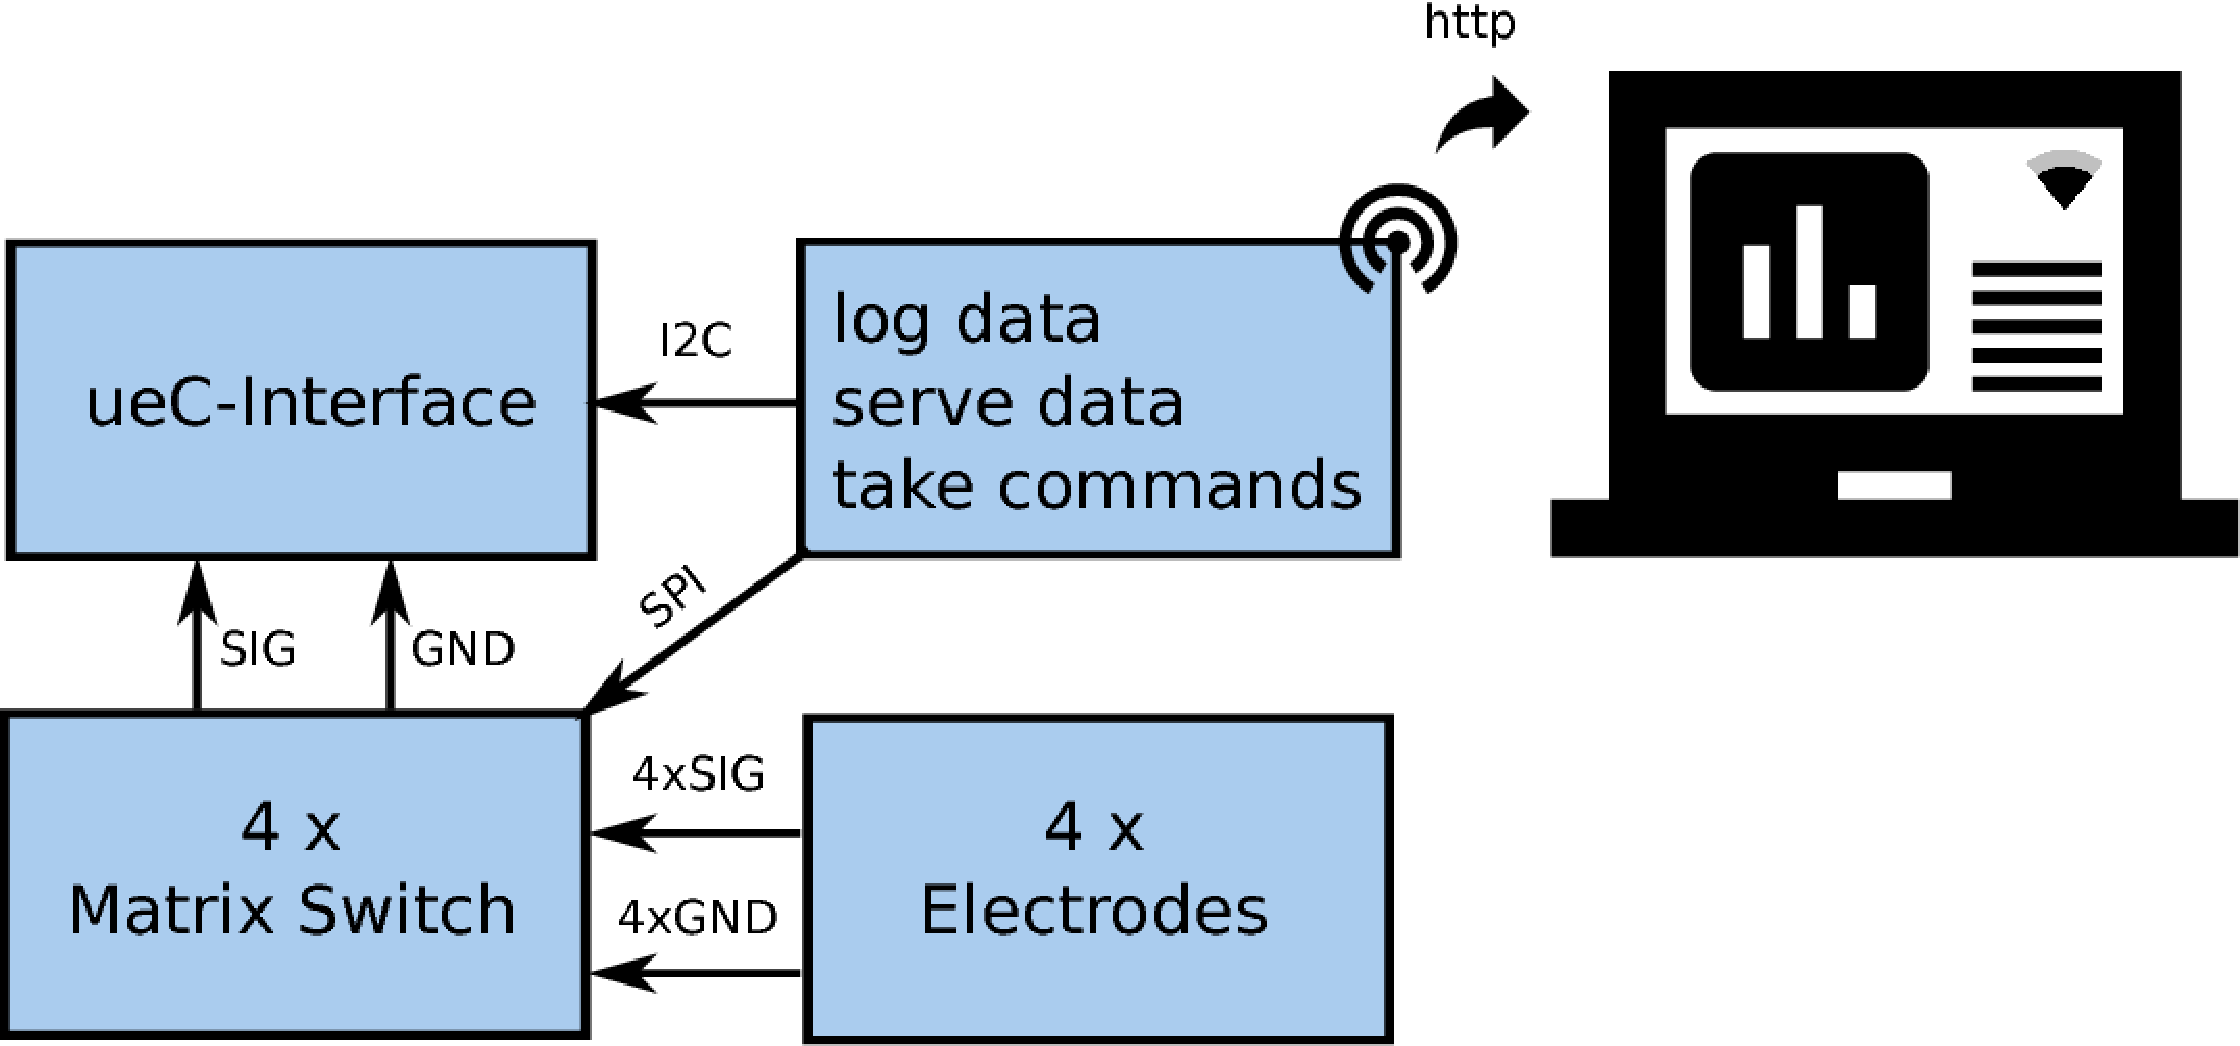
\includegraphics[width=\textwidth]{images/systemdesign.pdf} 
		\caption[System Design]{System Design - The yellow area marks the user interface of the system, the green area is the hardware that is mounted on the carrier board and the blue area shows the sensors deployed in the water stream. The rectangle marks the parts of the system that is repeated $n$ times to get to the needed number of sensors.}
		\label{fig:sys}
	\end{center}
\end{figure}

To add further sensors to the system, two strategies are possible:

\begin{itemize}
    \item by chaining up multiple stages of matrix switches, the number of electrodes can be increased eightfold with each stage
    \item by connecting another MinieC Interface with its own set of matrix switches to the microcontroller, 8 more electrodes can be added with each of these subsystems
\end{itemize}

The first option results in lower costs per added electrode pair, as the MinieC interface is shared. However, with such a system, all electrodes have to be read in series, while with the second option each MinieC interface can be read in parallel, resulting in a higher sample rate. Practically this option is also easier to achieve. For the first option, a board with 18 matrix switches and 80 connections is needed, while the second option only uses two switches per board resulting in 16 connections. The simpler board greatly reduces complexity and also can be made smaller.

\section{Electrodes}

The electrode pairs are the actual sensors in contact with the fluid to be measured. Their material and geometry influence the measuring range of the system. According to  \textcite{trankler2015sensortechnik} a cell constant $ C $ of $1$ enables a range from \unitfrac[$2 \cdot 10^3$]{$\mu S$}{cm} to \unitfrac[$10 \cdot 10^3$]{$\mu S$}{cm}. For a water temperature of \unit[$18^\circ$]{C}, this corresponds to salinities of \unit[0.12]{\%} and \unit[0.66]{\%}, which would be lower than those stated in the requirements. Still, a cell constant $ C $ of $1$ is the best compromise for our purpose. \textcite{trankler2015sensortechnik} do not specify the material's influence on the range and how the usable range is defined, leaving room for a possibly higher than anticipated range. First bench tests confirmed this assumption.\\

Figure \ref{fig:sensor} shows the geometry of the sensor. To achieve a cell constant $C$ of $1$, a width $w$ of \unit[1]{mm}, height $h$ of \unit[10]{mm} and distance $d$ of \unit[10]{mm} were chosen.\\

\begin{figure}[H]
	\begin{center}
		\begin{tikzpicture}
			\draw [line width=0.5mm] (-1,-1) -- (-1,1) -- (-1.3,1) -- (-1.3,-1) -- (-1,-1);
			\draw [dash dot] (-1.15,-1.5) -- (-1.15,1.2);
			\draw [line width=0.5mm] (1,-1) -- (1,1) -- (1.3,1) -- (1.3,-1) -- (1,-1);
			\draw [dash dot] (1.15,-1.5) -- (1.15,1.2);

			\draw (-1,1.6) -- (-1,1);
			\draw (-1.3,1.6) -- (-1.3,1);
			\draw (-1,1.4) -- (-1.3,1.4) node[above, pos=-0.75] {$w$};
			\draw [arrow]  (-1.7,1.4) -- (-1.3,1.4);
			\draw [arrow] (-0.6,1.4) -- (-1,1.4);
			
			\draw (-1.9,1) -- (-1.3,1);
			\draw (-1.9,-1) -- (-1.3,-1);
			\draw [darrow] (-1.7,1) -- (-1.7,-1) node[left, pos=0.5] {$h$};

			\draw [darrow] (-1.15,-1.3) -- (1.15,-1.3) node[below, pos=0.5] {$d$};

		\end{tikzpicture}
		\caption{Two rectangular electrodes form an electrode pair}
		\label{fig:sensor}
	\end{center}
\end{figure}

As a first proof-of-concept a sensor array was built, containing multiple electrode pairs on a strip, pictured in Figure \ref{fig:v2}. A \unit[50]{mm} wide and \unit[250]{mm} long band of Kapton adhesive tape served as the base. Four electrode pairs made from \unit[0.2]{mm} platinum wire were arranged equidistant on the strip. Eight \unit[0.4]{mm} enameled copper wires were run along the tape to connect each electrode to the left end of the strip, from which insulated cables connected to the carrier board. After soldering the joints, two smaller strips of tape were used to cover the wiring, exposing only the electrodes to the fluid.

First tests with this sensor array showed the viability of the concept, however a simple look at it shows the inherent problems: instead of a uniformly flat strip with minimal influence on the flow, the assembly forms several irregularities. Soldering \unit[0.2]{mm} platinum wire to \unit[0.4]{mm} enameled copper wire on a piece of adhesive tape per hand also did not result in clean solder joints. While, after the experience of the first array, the second array turned out a bit cleaner, the fundamental problem remains: it is a tedious manufacturing process resulting in a low quality product.

\begin{figure}[H]
	\begin{center}
		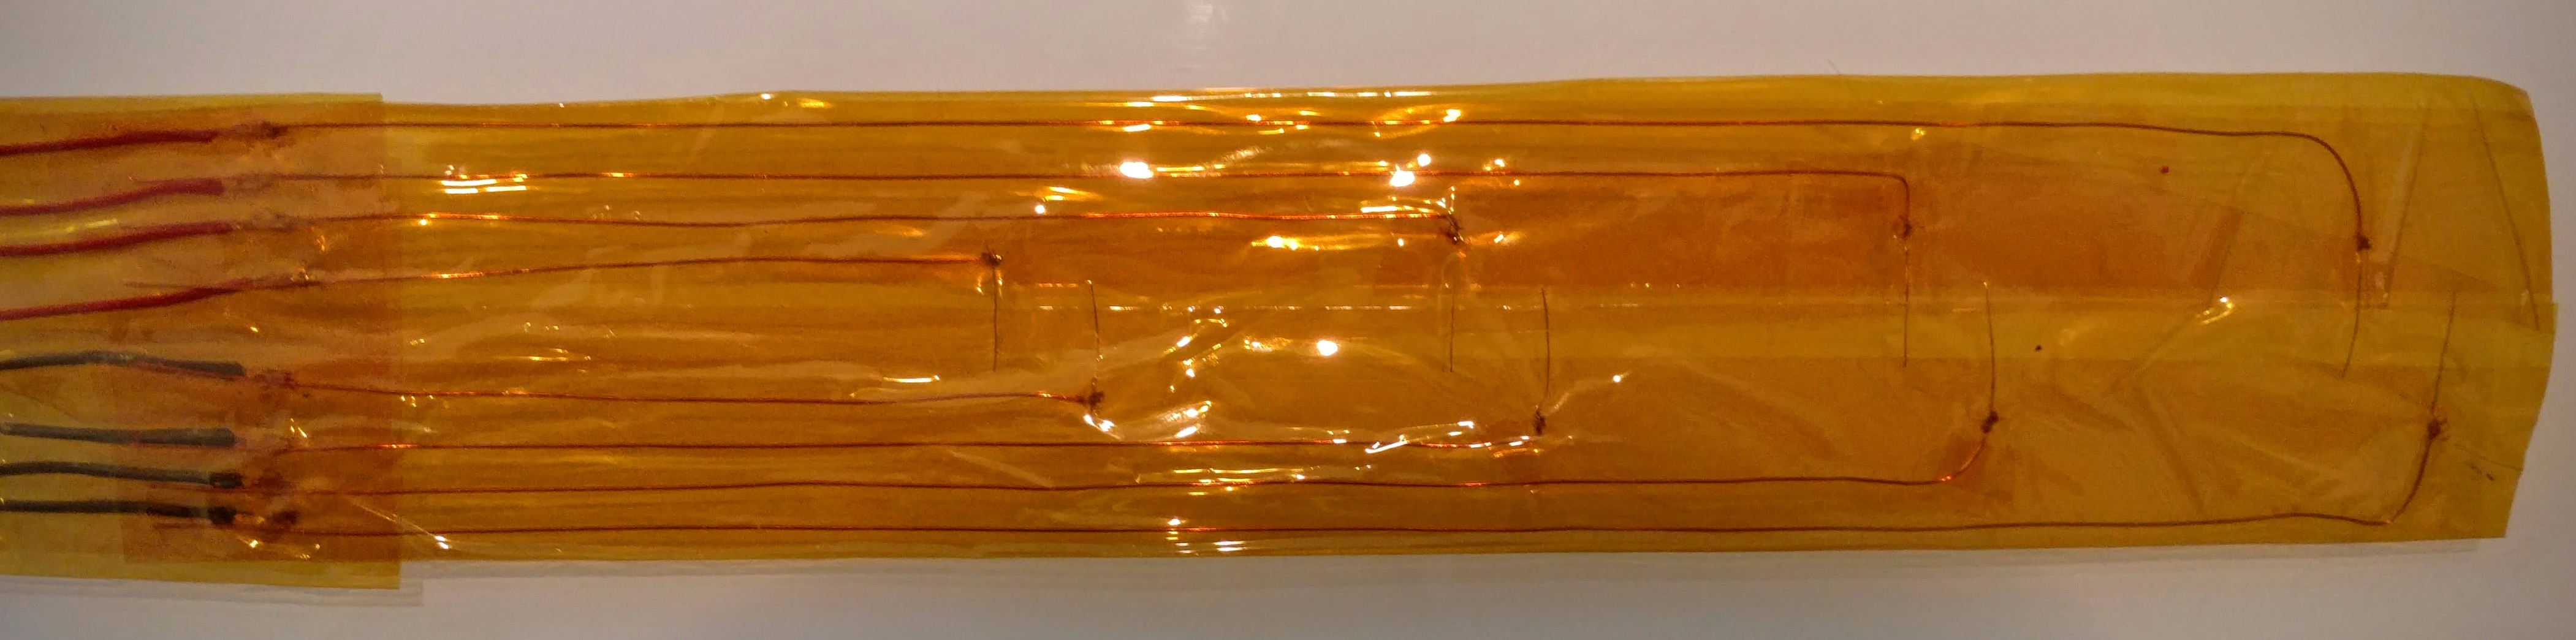
\includegraphics[width=\textwidth]{images/v2.jpg} 
		\caption[A handmade sensor strip]{A handmade sensor strip - The short, vertical silver lines are the platinum electrodes, the darker horizontal lines are the copper wires, running to the cables attached on the left.}
		\label{fig:v2}
	\end{center}
\end{figure}

As an alternative to these handmade strips, industrially produced flexible printed circuit boards (flex-PCB) were identified. These are constructed similar to the handmade arrays described above. They also use Kapton as a base, on which a copper coating is applied and partially removed by etching to form the conducting paths. On top, another layer of Kapton is applied, with cutouts in the places where the copper is supposed to be exposed. The exposed copper is then plated with ENIG (Electroless nickel immersion gold) to protect the copper from oxidation and provide the landing pads for electrical components to be soldered on.

For our purpose those exposed and plated landing pads can be used as electrodes, being nicely embedded in a flex-PCB that also runs the wiring up to an interface where cables can be connected. Using the flex-PCB itself as cable is not viable due to the high costs per area. The cables are soldered on directly and silicone is used to create a waterproof seal around the connection.\\

The final design for the sensor strip, as shown in Figure \ref{fig:fpcbd}, implemented as a flex-PCB consists of four electrode pairs spaced \unit[50]{mm} apart. The strip is \unit[25]{mm} wide and \unit[220]{mm} long. Figure \ref{fig:fpcbp} shows one of the 16 pieces that were manufactured by the company LEITON.

\begin{figure}[H]
	\begin{center}
		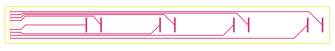
\includegraphics[width=\textwidth]{images/fpcbd.pdf} 
		\caption[The sensor strip design to be implemented as flex-PCB]{The sensor strip design to be implemented as a flex-PCB - The red lines mark the copper layer, the green line is the outline of the board.}
		\label{fig:fpcbd}
	\end{center}
\end{figure}

\begin{figure}[H]
	\begin{center}
		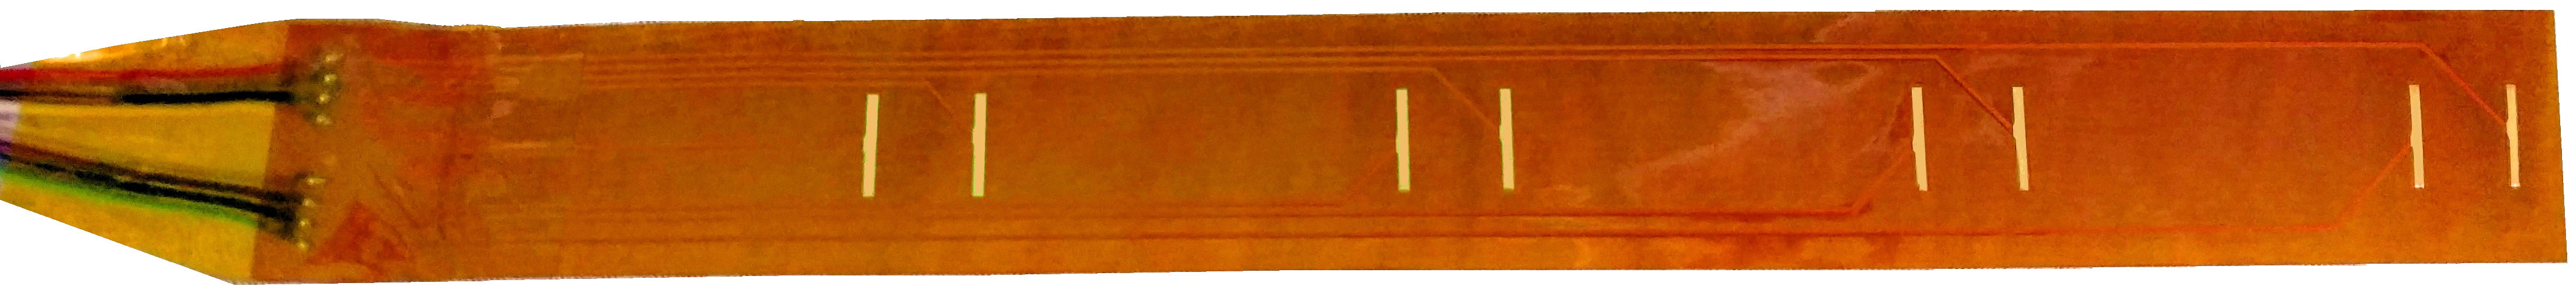
\includegraphics[width=\textwidth]{images/fpcbp.jpg} 
		\caption{A finished sensor strip assembled with cables and waterproofing on the left}
		\label{fig:fpcbp}
	\end{center}
\end{figure}

\section{Matrix Switches}

The matrix switches are an essential part of the system, enabling the use of multiple sensors with a single MinieC Interface, thus lowering the costs per sensor. The component used is an Analog Devices ADG738. It is an 8-channel CMOS analog matrix switch controlled via the SPI interface. The following information is taken from the data sheet provided by the manufacturer \textcite{ms}.\\

Figure \ref{fig:ms} shows the functional block diagram. The switch has one drain pin (D) and 8 source pins (S1 - S8). Despite the naming of drain and source, the internals provide simple switches between the drain and each source pin. The switches work in both directions without any restriction on the signal other than a maximum current of \unit[120]{mA}, which far exceeds our needs. By sending control commands via the SPI interface, each of the 8 internal switches can be turned on and off individually.\\

\begin{figure}[H]
	\begin{center}
		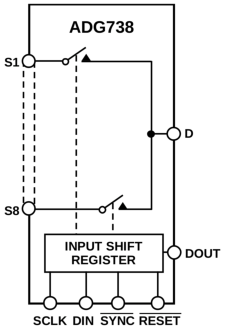
\includegraphics[width=0.3\textwidth]{images/ms.pdf} 
		\caption[The functional block diagram of the ADG738 matrix switch.]{The functional block diagram of the ADG738 matrix switch - Pin (D) is connected to the outputs (S1 - S2) via switches, that are controlled by SPI-input on (DIN). (SCLK) is driven by the clock, (SYNC) is the chip select pin and (RESET) breaks the connection of all switches. (DOUT) provides the signal of (DIN) to enable daisy-chaining \parencite{ms}.}
		\label{fig:ms}
	\end{center}
\end{figure}

The example timing diagram in Figure \ref{fig:msc} describes the data transmission process. The microcontroller sends one byte of data to the matrix switch. Each of the 8 bits of this byte controls one switch. The first bit controls the first switch and so on. If the bit is 1, the switch is closed; if it is 0, the switch is open. To send the byte, first the synchronization pin (SYNC) has to be pulled low from its usual high level. A clock signal is provided to the clock pin (SCLK). At each falling edge of the clock signal, the data input (DIN) is read - where a high signal leads to a 1-bit and a low signal to a 0-bit. After 8 cycles, SYNC is pulled high again marking the end of data transmission with a full byte transferred. Subsequently, the switches immediately take their instructed states with switching times in the order of \unit[100]{ns}. The complete process of transferring one byte and switching to the new state takes about \unit[520]{$\mu$s}.\\

\begin{figure}[H]
	\begin{center}
	\tikzexternaldisable
		\begin{tikztimingtable}
  			SYNC   & H 32{L} H \\
  			SCLK   & C 16{2C} N(A1) C \\
  			DIN  	& 2{L} {2H} N(B1) 15{2L} \\
  			Data	& 2D{} 2D{1} 2D{} 2D{0} 2D{} 2D{0} 2D{} 2D{0} 2D{} 2D{0} 2D{} 2D{0} 2D{} 2D{0} 2D{} 2D{0} 2D{}\\
		\end{tikztimingtable}
		\caption[Example Timing Diagram]{Example Timing Diagram - Data input starts when (SYNC) is pulled low. On falling edges of (SCLK), (DIN) is read. If (DIN) is high at that moment, the bit is 1, if low it is 0. After eight bits are transferred, (SYNC) is pulled high again and the data transfer is finished. The resulting state is a closed first switch while all other switches are open.}
		\label{fig:msc}
	\end{center}
\end{figure}

Multiple matrix switches can be controlled at once by daisy-chaining the data output pin (DOUT) of the first device to DIN of the second one, and so forth. Both SYNC and SCLK are connected to the same bus. This assures that all matrix switches are set in the same state and at the same time which is important for our case to synchronize the two used ADG738 parts.

\section{MinieC Interface}

The MinieC Interface contains the electronics to perform the resistance measurement. It contains several parts used to generate an analog signal, to run it through a circuit in which the liquid to be measured serves as a resistor and to measure the voltage drop over it.\\

The first part is a charge pump voltage inverter. Its purpose is to generate a negative output voltage from a positive input. The negative voltage and the positive voltage are needed to drive a Wien bridge oscillator. This oscillator outputs a sine wave voltage oscillating between the positive and negative input voltage. The purpose of the first stage is to generate an alternating current (AC) to be used in the measurement, avoiding the polarization effects mentioned before.\\

The AC signal provided by the first stage is then fed into an operational amplifier (opamp). An opamp is a device that has two input signals and one output, where the output is proportional to the difference of the input signals. In our case, the opamp's output is pulled to ground via a voltage divider as shown in Figure \ref{fig:opamp}. The first resistor $R_i$ in the divider is fixed, while the second resistor $R$ is the liquid to be measured. The output voltage of this divider is dependent on the liquid's resistance. This voltage is then fed back into the second input of the opamp. Via this feedback, the output (OUT) of the opamp is now the input signal (SIG) modulated in amplitude by the resistance of the liquid.

\begin{figure}[H]
	\begin{center}
		\begin{circuitikz}
			\draw
				(0,0) node[op amp, yscale=-1](oa1) {}
				(0,0) node[] {OA}
				(oa1.+) node[left] {SIG}
				(oa1.out) to[R=$R_i$] +(0,-2) coordinate (fb)
			    to[vR=$R$] +(0,-2)
			    to +(0,0) node[ground] {}
			   (fb) to[short, o-] +(-3,2) coordinate (i1)
			   (oa1.-) to[short] +(0,1.5) coordinate (i2)
			   (i1) to (i2)
			   (oa1.out) to[short, o-] +(1,0) coordinate (out)
			   (out) node[right] {OUT}
				;
		\end{circuitikz}
		\caption[The opamp (OA) modulates the input signals (SIG) amplitude.]{The opamp (OA) modulates the input signals (SIG) amplitude proportional to the variable resistance $R$ in the voltage divider to generate the output (OUT)}
		\label{fig:opamp}
	\end{center}
\end{figure}

In the last step, the modulated output is amplified in two stages, filtered, and then measured by an analog-digital-converter (ADC). The ADC measures the voltage and provides the measurement to the microcontroller via I2C.\\

First tests of the interface surfaced an interesting problem. The graph displayed in figure \ref{fig:swcap} shows the response to an immediate switch from the AC input signal to zero. The first red line marks the moment of the switch, the second line marks the moment when the response reached the voltage zero. It took \unit[40]{ms} for the response to follow the input. This slow response time is not acceptable for our system because it prohibits the rapid switching between sensors needed for the fast sampling of data. It would smear the measurement over all sensors and it would not be possible to sense a difference between them. Waiting for that amount of time between each read of a sensor would reduce the time resolution to a level where the desired information can no longer be extracted from the data. The cause of this behavior is the filter placed before the ADC. As the output of the opamp is an alternating current, a diode and a filter capacitor are used to generate a direct current signal proportional to the amplitude of the AC signal. This is done so that the sample rate of the ADC does not have to match the frequency of the signal, which makes it easier to use when fast sampling rates are not necessary.\\

\begin{figure}[H]
	\begin{center}
		% This file was created by matplotlib2tikz v0.5.10.
\begin{tikzpicture}

\begin{axis}[
xlabel={Time, s},
ylabel={Voltage, V},
xmin=0, xmax=0.8,
ymin=0, ymax=1,
axis on top,
xtick={0,0.1,0.2,0.3,0.4,0.5,0.6,0.7,0.8},
xticklabels={0.0,0.1,0.2,0.3,0.4,0.5,0.6,0.7,0.8},
ytick={0,0.2,0.4,0.6,0.8,1},
yticklabels={0.0,0.2,0.4,0.6,0.8,1.0}
]
\addplot [draw=blue, fill=blue, opacity=0.5, mark=*, only marks] table {%
0.0 0.927734375
0.0 0.886962890625
0.001 0.936767578125
0.001 0.90234375
0.001 0.935302734375
0.001 0.907958984375
0.002 0.92919921875
0.002 0.9111328125
0.002 0.921875
0.002 0.92041015625
0.003 0.8857421875
0.003 0.929443359375
0.003 0.890625
0.004 0.939453125
0.004 0.891845703125
0.004 0.938232421875
0.004 0.90283203125
0.005 0.933837890625
0.005 0.906982421875
0.005 0.929931640625
0.006 0.915771484375
0.006 0.923095703125
0.006 0.919189453125
0.006 0.900390625
0.007 0.927001953125
0.007 0.884033203125
0.007 0.930419921875
0.008 0.890380859375
0.008 0.93701171875
0.008 0.894775390625
0.008 0.937744140625
0.009 0.902587890625
0.009 0.937744140625
0.009 0.905517578125
0.009 0.932861328125
0.01 0.909423828125
0.01 0.930419921875
0.01 0.913818359375
0.011 0.917724609375
0.011 0.91552734375
0.011 0.90966796875
0.011 0.923095703125
0.012 0.89697265625
0.012 0.92724609375
0.012 0.887451171875
0.013 0.933349609375
0.013 0.888427734375
0.013 0.93603515625
0.014 0.89453125
0.014 0.935302734375
0.014 0.894287109375
0.014 0.938232421875
0.015 0.901123046875
0.015 0.938720703125
0.015 0.906005859375
0.016 0.934326171875
0.016 0.903564453125
0.016 0.933349609375
0.016 0.90966796875
0.017 0.930419921875
0.017 0.912353515625
0.017 0.925537109375
0.018 0.916748046875
0.018 0.926513671875
0.018 0.916748046875
0.018 0.916259765625
0.019 0.919189453125
0.019 0.91357421875
0.019 0.921875
0.02 0.891357421875
0.02 0.922119140625
0.02 0.89404296875
0.021 0.926025390625
0.021 0.900634765625
0.021 0.92529296875
0.021 0.884521484375
0.022 0.927978515625
0.022 0.886474609375
0.022 0.926513671875
0.023 0.885009765625
0.023 0.926513671875
0.023 0.8857421875
0.024 0.9296875
0.024 0.883544921875
0.024 0.927001953125
0.024 0.885009765625
0.025 0.927734375
0.025 0.884521484375
0.025 0.929443359375
0.026 0.886474609375
0.026 0.929931640625
0.026 0.887451171875
0.027 0.930419921875
0.027 0.883544921875
0.027 0.92822265625
0.027 0.885498046875
0.028 0.924072265625
0.028 0.884521484375
0.028 0.927734375
0.029 0.885498046875
0.029 0.926513671875
0.029 0.885498046875
0.03 0.926513671875
0.03 0.903564453125
0.03 0.923828125
0.031 0.896240234375
0.031 0.916748046875
0.031 0.91552734375
0.031 0.919677734375
0.032 0.923583984375
0.032 0.915771484375
0.032 0.925048828125
0.033 0.916748046875
0.033 0.927978515625
0.033 0.913330078125
0.034 0.927978515625
0.034 0.907958984375
0.034 0.933349609375
0.035 0.908203125
0.035 0.937255859375
0.035 0.90478515625
0.035 0.937255859375
0.036 0.8984375
0.036 0.939208984375
0.036 0.900146484375
0.037 0.9404296875
0.037 0.894287109375
0.037 0.94140625
0.038 0.896484375
0.038 0.937744140625
0.038 0.892822265625
0.039 0.93603515625
0.039 0.886962890625
0.039 0.927978515625
0.04 0.884521484375
0.04 0.919677734375
0.04 0.916259765625
0.041 0.91845703125
0.041 0.930419921875
0.041 0.911376953125
0.041 0.932373046875
0.042 0.90283203125
0.042 0.9375
0.042 0.903564453125
0.043 0.939208984375
0.043 0.89794921875
0.043 0.941162109375
0.044 0.89453125
0.044 0.935302734375
0.044 0.889892578125
0.045 0.932373046875
0.045 0.891845703125
0.045 0.923583984375
0.046 0.909912109375
0.046 0.919677734375
0.046 0.92529296875
0.047 0.913818359375
0.047 0.93603515625
0.047 0.90673828125
0.048 0.937744140625
0.048 0.899169921875
0.048 0.941162109375
0.049 0.897216796875
0.049 0.935302734375
0.049 0.889404296875
0.05 0.928955078125
0.05 0.913330078125
0.05 0.918701171875
0.051 0.925537109375
0.051 0.90771484375
0.051 0.936279296875
0.051 0.904541015625
0.052 0.940185546875
0.052 0.898681640625
0.052 0.941162109375
0.053 0.887451171875
0.053 0.927490234375
0.053 0.899658203125
0.054 0.916259765625
0.054 0.930419921875
0.054 0.910400390625
0.055 0.936279296875
0.055 0.902099609375
0.055 0.941162109375
0.056 0.891845703125
0.056 0.934326171875
0.056 0.887451171875
0.057 0.919189453125
0.057 0.925048828125
0.057 0.913818359375
0.058 0.936767578125
0.058 0.904052734375
0.058 0.940673828125
0.059 0.892333984375
0.059 0.935302734375
0.059 0.887939453125
0.06 0.919189453125
0.06 0.926025390625
0.06 0.911865234375
0.061 0.939208984375
0.061 0.902099609375
0.062 0.94189453125
0.062 0.891845703125
0.062 0.931396484375
0.063 0.893310546875
0.063 0.91650390625
0.063 0.932373046875
0.064 0.907958984375
0.064 0.941162109375
0.064 0.899169921875
0.065 0.941162109375
0.065 0.888427734375
0.065 0.924560546875
0.066 0.921142578125
0.066 0.91064453125
0.066 0.937255859375
0.067 0.90234375
0.067 0.942626953125
0.067 0.89599609375
0.068 0.93603515625
0.068 0.888427734375
0.068 0.923583984375
0.069 0.927490234375
0.069 0.907958984375
0.069 0.940185546875
0.07 0.901123046875
0.07 0.938720703125
0.07 0.889892578125
0.071 0.92578125
0.071 0.927490234375
0.071 0.910888671875
0.072 0.938720703125
0.072 0.898681640625
0.072 0.941162109375
0.073 0.887451171875
0.073 0.922607421875
0.073 0.928466796875
0.074 0.905029296875
0.074 0.941162109375
0.075 0.897705078125
0.075 0.93408203125
0.075 0.899658203125
0.076 0.919677734375
0.076 0.936767578125
0.076 0.902587890625
0.077 0.9443359375
0.077 0.890380859375
0.077 0.927490234375
0.078 0.928466796875
0.078 0.910888671875
0.078 0.939697265625
0.079 0.893798828125
0.079 0.936767578125
0.079 0.889892578125
0.08 0.915771484375
0.08 0.936767578125
0.08 0.903076171875
0.081 0.942138671875
0.081 0.891357421875
0.082 0.9267578125
0.082 0.93310546875
0.082 0.906982421875
0.083 0.945068359375
0.083 0.892333984375
0.083 0.932373046875
0.084 0.923583984375
0.084 0.912353515625
0.084 0.939697265625
0.085 0.892333984375
0.085 0.935546875
0.085 0.90478515625
0.086 0.9130859375
0.086 0.939208984375
0.087 0.898681640625
0.087 0.93896484375
0.087 0.891357421875
0.088 0.921142578125
0.088 0.937255859375
0.088 0.902099609375
0.089 0.93701171875
0.089 0.887939453125
0.089 0.921630859375
0.09 0.938720703125
0.09 0.901123046875
0.091 0.943115234375
0.091 0.893798828125
0.091 0.9208984375
0.092 0.941162109375
0.092 0.899169921875
0.092 0.943359375
0.093 0.89892578125
0.093 0.91845703125
0.093 0.937255859375
0.094 0.896240234375
0.094 0.939453125
0.095 0.894287109375
0.095 0.91552734375
0.095 0.939697265625
0.096 0.898681640625
0.096 0.93408203125
0.096 0.915771484375
0.097 0.90869140625
0.097 0.942626953125
0.097 0.895263671875
0.098 0.927490234375
0.098 0.930419921875
0.099 0.9091796875
0.099 0.943603515625
0.099 0.89208984375
0.1 0.92333984375
0.1 0.934326171875
0.1 0.904052734375
0.101 0.94091796875
0.101 0.892822265625
0.102 0.919677734375
0.102 0.9404296875
0.102 0.897216796875
0.103 0.931396484375
0.103 0.925537109375
0.103 0.910400390625
0.104 0.944091796875
0.104 0.892333984375
0.105 0.924560546875
0.105 0.938232421875
0.105 0.90087890625
0.106 0.933837890625
0.106 0.918701171875
0.106 0.912841796875
0.107 0.943603515625
0.107 0.893310546875
0.108 0.926513671875
0.108 0.935791015625
0.108 0.901611328125
0.109 0.932373046875
0.109 0.909912109375
0.109 0.914794921875
0.11 0.94384765625
0.11 0.8935546875
0.111 0.927490234375
0.111 0.934326171875
0.111 0.902587890625
0.112 0.935302734375
0.112 0.909423828125
0.112 0.913818359375
0.113 0.94384765625
0.113 0.892822265625
0.114 0.9287109375
0.114 0.935302734375
0.114 0.90185546875
0.115 0.933349609375
0.115 0.918701171875
0.115 0.911865234375
0.116 0.945068359375
0.116 0.89013671875
0.117 0.916748046875
0.117 0.940673828125
0.117 0.895263671875
0.118 0.925048828125
0.118 0.935302734375
0.119 0.903564453125
0.119 0.938232421875
0.119 0.917236328125
0.12 0.906005859375
0.12 0.944091796875
0.12 0.889404296875
0.121 0.916259765625
0.121 0.941650390625
0.122 0.888671875
0.122 0.923583984375
0.122 0.9375
0.123 0.894287109375
0.123 0.9326171875
0.124 0.935546875
0.124 0.901611328125
0.124 0.940185546875
0.125 0.927734375
0.125 0.907470703125
0.126 0.947265625
0.126 0.903076171875
0.126 0.915283203125
0.127 0.943115234375
0.127 0.889892578125
0.128 0.920654296875
0.128 0.941162109375
0.128 0.893310546875
0.129 0.921630859375
0.129 0.938720703125
0.129 0.89697265625
0.13 0.928955078125
0.13 0.935302734375
0.131 0.894287109375
0.131 0.933349609375
0.131 0.930419921875
0.132 0.90087890625
0.132 0.9384765625
0.133 0.92919921875
0.133 0.90478515625
0.133 0.940673828125
0.134 0.927978515625
0.134 0.90576171875
0.135 0.934814453125
0.135 0.921630859375
0.135 0.908935546875
0.136 0.941162109375
0.136 0.913818359375
0.137 0.906494140625
0.137 0.943115234375
0.137 0.904052734375
0.138 0.908447265625
0.138 0.944580078125
0.139 0.916748046875
0.139 0.91064453125
0.139 0.945068359375
0.14 0.914794921875
0.14 0.9111328125
0.141 0.938720703125
0.141 0.909912109375
0.141 0.912353515625
0.142 0.942626953125
0.142 0.909912109375
0.143 0.906005859375
0.143 0.943115234375
0.143 0.910400390625
0.144 0.907958984375
0.144 0.942626953125
0.145 0.925537109375
0.145 0.906005859375
0.146 0.942138671875
0.146 0.918701171875
0.146 0.90966796875
0.147 0.938232421875
0.147 0.923095703125
0.148 0.90966796875
0.148 0.940185546875
0.148 0.92333984375
0.149 0.902099609375
0.149 0.93798828125
0.15 0.93359375
0.15 0.901123046875
0.15 0.935302734375
0.151 0.937255859375
0.151 0.897216796875
0.152 0.925537109375
0.152 0.93896484375
0.152 0.894287109375
0.153 0.923583984375
0.153 0.94091796875
0.154 0.88623046875
0.154 0.918701171875
0.155 0.944091796875
0.155 0.887451171875
0.155 0.917236328125
0.156 0.945068359375
0.156 0.904541015625
0.157 0.910400390625
0.157 0.941650390625
0.157 0.918701171875
0.158 0.903076171875
0.158 0.93798828125
0.159 0.93408203125
0.159 0.898193359375
0.159 0.931396484375
0.16 0.93896484375
0.16 0.893310546875
0.161 0.918701171875
0.161 0.942138671875
0.162 0.890869140625
0.162 0.914794921875
0.162 0.944091796875
0.163 0.92236328125
0.163 0.906005859375
0.164 0.928466796875
0.164 0.933349609375
0.165 0.900146484375
0.165 0.92822265625
0.165 0.9404296875
0.166 0.887939453125
0.166 0.91748046875
0.167 0.941162109375
0.167 0.912353515625
0.167 0.908935546875
0.168 0.936767578125
0.168 0.93212890625
0.169 0.895263671875
0.169 0.927490234375
0.17 0.939208984375
0.17 0.887939453125
0.17 0.91650390625
0.171 0.942626953125
0.171 0.920654296875
0.172 0.901123046875
0.172 0.933349609375
0.173 0.9345703125
0.173 0.892333984375
0.173 0.921630859375
0.174 0.944091796875
0.174 0.907958984375
0.175 0.905029296875
0.175 0.936279296875
0.176 0.93408203125
0.176 0.894287109375
0.176 0.925048828125
0.177 0.943115234375
0.177 0.899169921875
0.178 0.906494140625
0.178 0.937255859375
0.179 0.934326171875
0.179 0.894287109375
0.179 0.924560546875
0.18 0.94287109375
0.18 0.895263671875
0.181 0.90673828125
0.181 0.93701171875
0.182 0.935791015625
0.182 0.892822265625
0.182 0.9248046875
0.183 0.943115234375
0.183 0.909912109375
0.184 0.903076171875
0.184 0.934326171875
0.185 0.939697265625
0.185 0.890380859375
0.186 0.9169921875
0.186 0.942626953125
0.186 0.923095703125
0.187 0.898193359375
0.187 0.929443359375
0.188 0.943115234375
0.188 0.889892578125
0.189 0.905517578125
0.189 0.9375
0.189 0.935302734375
0.19 0.893310546875
0.19 0.92431640625
0.191 0.944580078125
0.191 0.915771484375
0.192 0.900634765625
0.192 0.93115234375
0.193 0.939453125
0.193 0.885986328125
0.193 0.912353515625
0.194 0.936279296875
0.194 0.935302734375
0.195 0.889404296875
0.195 0.91748046875
0.196 0.939453125
0.196 0.93017578125
0.197 0.89599609375
0.197 0.9248046875
0.197 0.942138671875
0.198 0.919189453125
0.198 0.903564453125
0.199 0.928466796875
0.199 0.941162109375
0.2 0.907470703125
0.2 0.906982421875
0.201 0.929443359375
0.201 0.940185546875
0.201 0.886962890625
0.202 0.911865234375
0.202 0.938232421875
0.203 0.938232421875
0.203 0.89013671875
0.204 0.911376953125
0.204 0.939208984375
0.207 0.93505859375
0.207 0.906494140625
0.207 0.93017578125
0.207 0.916259765625
0.208 0.919921875
0.208 0.923583984375
0.208 0.884521484375
0.209 0.93359375
0.209 0.887451171875
0.209 0.93896484375
0.209 0.897216796875
0.21 0.93798828125
0.21 0.903076171875
0.21 0.932861328125
0.21 0.9130859375
0.211 0.927734375
0.211 0.915771484375
0.211 0.9130859375
0.212 0.924072265625
0.212 0.883544921875
0.212 0.9306640625
0.212 0.890380859375
0.213 0.93359375
0.213 0.892822265625
0.213 0.938232421875
0.214 0.902587890625
0.214 0.937744140625
0.214 0.90625
0.214 0.932373046875
0.215 0.909423828125
0.215 0.927734375
0.215 0.915771484375
0.216 0.91162109375
0.216 0.91796875
0.216 0.900634765625
0.216 0.926025390625
0.217 0.884033203125
0.217 0.9306640625
0.217 0.890380859375
0.218 0.9384765625
0.218 0.891845703125
0.218 0.939208984375
0.218 0.898193359375
0.219 0.936279296875
0.219 0.899658203125
0.219 0.93701171875
0.22 0.905517578125
0.22 0.936279296875
0.22 0.908203125
0.22 0.930908203125
0.221 0.906005859375
0.221 0.929443359375
0.221 0.913818359375
0.222 0.921630859375
0.222 0.915283203125
0.222 0.919189453125
0.222 0.920654296875
0.223 0.919677734375
0.223 0.919921875
0.223 0.897216796875
0.224 0.922119140625
0.224 0.896728515625
0.224 0.926025390625
0.225 0.884033203125
0.225 0.926513671875
0.225 0.884521484375
0.225 0.929931640625
0.226 0.881591796875
0.226 0.929443359375
0.226 0.887451171875
0.227 0.93505859375
0.227 0.88818359375
0.227 0.934326171875
0.228 0.891845703125
0.228 0.933837890625
0.228 0.890380859375
0.228 0.93701171875
0.229 0.886962890625
0.229 0.933837890625
0.229 0.890380859375
0.23 0.937744140625
0.23 0.890380859375
0.23 0.9375
0.231 0.892333984375
0.231 0.934326171875
0.231 0.891357421875
0.231 0.936279296875
0.232 0.886474609375
0.232 0.932373046875
0.232 0.889404296875
0.233 0.928466796875
0.233 0.885986328125
0.233 0.931640625
0.234 0.89013671875
0.234 0.929443359375
0.234 0.885986328125
0.235 0.929931640625
0.235 0.887939453125
0.235 0.925537109375
0.235 0.886474609375
0.236 0.917724609375
0.236 0.913818359375
0.236 0.919677734375
0.237 0.925048828125
0.237 0.913818359375
0.237 0.927001953125
0.238 0.913818359375
0.238 0.933349609375
0.238 0.908447265625
0.239 0.935302734375
0.239 0.905029296875
0.239 0.935791015625
0.239 0.905029296875
0.24 0.940185546875
0.24 0.902099609375
0.24 0.939697265625
0.241 0.895263671875
0.241 0.94140625
0.241 0.894287109375
0.242 0.9306640625
0.242 0.886962890625
0.242 0.931640625
0.243 0.9013671875
0.243 0.9228515625
0.243 0.9130859375
0.244 0.91552734375
0.244 0.92919921875
0.244 0.911865234375
0.245 0.938232421875
0.245 0.904052734375
0.245 0.937744140625
0.246 0.902099609375
0.246 0.940673828125
0.246 0.900146484375
0.247 0.940673828125
0.247 0.893798828125
0.247 0.937255859375
0.247 0.890869140625
0.248 0.926513671875
0.248 0.900146484375
0.248 0.922119140625
0.249 0.928955078125
0.249 0.912841796875
0.249 0.932861328125
0.25 0.902099609375
0.25 0.939453125
0.25 0.901611328125
0.251 0.941162109375
0.251 0.8955078125
0.251 0.938232421875
0.252 0.884521484375
0.252 0.925537109375
0.252 0.905029296875
0.253 0.914306640625
0.253 0.9306640625
0.253 0.909912109375
0.254 0.936279296875
0.254 0.902099609375
0.254 0.94091796875
0.255 0.892822265625
0.255 0.937255859375
0.255 0.89013671875
0.256 0.923583984375
0.256 0.915283203125
0.256 0.917724609375
0.257 0.932373046875
0.257 0.9072265625
0.257 0.938232421875
0.258 0.897216796875
0.258 0.942626953125
0.258 0.894287109375
0.259 0.928466796875
0.259 0.895751953125
0.259 0.921630859375
0.26 0.929443359375
0.26 0.909423828125
0.26 0.9375
0.261 0.897216796875
0.261 0.942138671875
0.261 0.894287109375
0.262 0.927490234375
0.262 0.897705078125
0.262 0.921630859375
0.263 0.931396484375
0.263 0.908935546875
0.263 0.938232421875
0.264 0.89599609375
0.264 0.942138671875
0.264 0.893310546875
0.265 0.92626953125
0.265 0.913818359375
0.265 0.917724609375
0.266 0.936279296875
0.266 0.904541015625
0.266 0.941162109375
0.267 0.892822265625
0.267 0.935302734375
0.267 0.887451171875
0.268 0.917724609375
0.268 0.931884765625
0.268 0.908203125
0.269 0.94189453125
0.269 0.897216796875
0.27 0.939208984375
0.27 0.88818359375
0.27 0.924072265625
0.271 0.925048828125
0.271 0.911865234375
0.271 0.93798828125
0.272 0.904296875
0.272 0.943359375
0.272 0.893310546875
0.273 0.932373046875
0.273 0.919189453125
0.273 0.914794921875
0.274 0.935546875
0.274 0.90087890625
0.274 0.943603515625
0.275 0.887451171875
0.275 0.92529296875
0.275 0.924560546875
0.276 0.906494140625
0.276 0.940673828125
0.276 0.898193359375
0.277 0.936279296875
0.277 0.89208984375
0.277 0.921142578125
0.278 0.936279296875
0.278 0.904052734375
0.279 0.942138671875
0.279 0.894287109375
0.279 0.934326171875
0.28 0.899169921875
0.28 0.918701171875
0.28 0.935791015625
0.281 0.902099609375
0.281 0.942626953125
0.281 0.892822265625
0.282 0.923583984375
0.282 0.927978515625
0.282 0.910888671875
0.283 0.94189453125
0.283 0.896240234375
0.283 0.935302734375
0.284 0.920654296875
0.284 0.913818359375
0.284 0.938232421875
0.285 0.897216796875
0.285 0.941162109375
0.286 0.896240234375
0.286 0.921875
0.286 0.933349609375
0.287 0.900146484375
0.287 0.943603515625
0.287 0.892333984375
0.288 0.91943359375
0.288 0.93212890625
0.288 0.906982421875
0.289 0.943603515625
0.289 0.892333984375
0.289 0.927978515625
0.29 0.927490234375
0.29 0.909912109375
0.291 0.94189453125
0.291 0.891357421875
0.291 0.932373046875
0.292 0.928466796875
0.292 0.909423828125
0.292 0.941650390625
0.293 0.891845703125
0.293 0.929443359375
0.293 0.925048828125
0.294 0.907958984375
0.294 0.942138671875
0.295 0.8955078125
0.295 0.928466796875
0.295 0.927001953125
0.296 0.904052734375
0.296 0.943115234375
0.296 0.892333984375
0.297 0.923095703125
0.297 0.934814453125
0.297 0.90576171875
0.298 0.941650390625
0.298 0.888916015625
0.299 0.915771484375
0.299 0.939208984375
0.299 0.89990234375
0.3 0.935302734375
0.3 0.915771484375
0.3 0.913818359375
0.301 0.942138671875
0.301 0.894287109375
0.302 0.931396484375
0.302 0.92919921875
0.302 0.90771484375
0.303 0.94482421875
0.303 0.8916015625
0.303 0.9248046875
0.304 0.939208984375
0.304 0.899169921875
0.305 0.939208984375
0.305 0.917724609375
0.305 0.91357421875
0.306 0.942626953125
0.306 0.89404296875
0.306 0.928466796875
0.307 0.936279296875
0.307 0.90185546875
0.308 0.9404296875
0.308 0.903564453125
0.308 0.916748046875
0.309 0.94189453125
0.309 0.894287109375
0.309 0.930419921875
0.31 0.934814453125
0.31 0.903076171875
0.311 0.938232421875
0.311 0.90576171875
0.311 0.915771484375
0.312 0.943115234375
0.312 0.893798828125
0.312 0.927978515625
0.313 0.934326171875
0.313 0.90283203125
0.314 0.935546875
0.314 0.910888671875
0.314 0.913818359375
0.315 0.944091796875
0.315 0.891357421875
0.315 0.925537109375
0.316 0.938232421875
0.316 0.898681640625
0.317 0.929443359375
0.317 0.92822265625
0.317 0.906982421875
0.318 0.94189453125
0.318 0.897705078125
0.319 0.910400390625
0.319 0.942626953125
0.319 0.892333984375
0.32 0.921630859375
0.32 0.938232421875
0.32 0.898193359375
0.321 0.933349609375
0.321 0.928955078125
0.322 0.901611328125
0.322 0.941162109375
0.322 0.904541015625
0.323 0.911376953125
0.323 0.943603515625
0.324 0.886474609375
0.324 0.918212890625
0.324 0.940673828125
0.325 0.890380859375
0.325 0.925537109375
0.326 0.936279296875
0.326 0.896240234375
0.326 0.933349609375
0.327 0.936767578125
0.327 0.89990234375
0.328 0.939453125
0.328 0.928466796875
0.328 0.906005859375
0.329 0.939697265625
0.329 0.916748046875
0.329 0.9130859375
0.33 0.94384765625
0.33 0.88916015625
0.331 0.913818359375
0.331 0.943359375
0.331 0.89111328125
0.332 0.9228515625
0.332 0.93994140625
0.333 0.886474609375
0.333 0.925537109375
0.333 0.937255859375
0.334 0.893798828125
0.334 0.930419921875
0.335 0.936279296875
0.335 0.898193359375
0.335 0.9345703125
0.336 0.936279296875
0.336 0.899169921875
0.337 0.924072265625
0.337 0.933349609375
0.337 0.901123046875
0.338 0.933837890625
0.338 0.931640625
0.339 0.896240234375
0.339 0.935302734375
0.339 0.928955078125
0.34 0.899169921875
0.34 0.937255859375
0.341 0.93310546875
0.341 0.901611328125
0.341 0.9384765625
0.342 0.932373046875
0.342 0.902099609375
0.343 0.931396484375
0.343 0.931396484375
0.343 0.902099609375
0.344 0.937255859375
0.344 0.927490234375
0.345 0.899658203125
0.345 0.937255859375
0.345 0.930419921875
0.346 0.902587890625
0.346 0.939453125
0.347 0.932861328125
0.347 0.902099609375
0.347 0.939453125
0.348 0.930419921875
0.348 0.903076171875
0.349 0.933837890625
0.349 0.932373046875
0.349 0.902099609375
0.35 0.93212890625
0.35 0.9345703125
0.351 0.894287109375
0.351 0.929443359375
0.352 0.93701171875
0.352 0.893310546875
0.352 0.9267578125
0.353 0.941162109375
0.353 0.89111328125
0.354 0.915771484375
0.354 0.943115234375
0.354 0.887939453125
0.355 0.916748046875
0.355 0.943603515625
0.356 0.909912109375
0.356 0.910888671875
0.356 0.943359375
%0.357 0.814208984375
0.358 0.765380859375
0.358 0.739990234375
0.359 0.71484375
0.359 0.687744140625
0.359 0.665771484375
0.359 0.644287109375
0.36 0.6240234375
0.36 0.602294921875
0.36 0.58349609375
0.36 0.565673828125
0.361 0.545654296875
0.361 0.52978515625
0.361 0.5146484375
0.362 0.499755859375
0.362 0.4833984375
0.362 0.469482421875
0.362 0.4560546875
0.363 0.440185546875
0.363 0.428955078125
0.363 0.416748046875
0.364 0.405029296875
0.364 0.393310546875
0.364 0.38232421875
0.364 0.371826171875
0.365 0.360107421875
0.365 0.350830078125
0.365 0.34130859375
0.365 0.331787109375
0.366 0.32177734375
0.366 0.313232421875
0.366 0.30517578125
0.367 0.2958984375
0.367 0.2880859375
0.367 0.280029296875
0.367 0.2724609375
0.368 0.264404296875
0.368 0.25732421875
0.368 0.25048828125
0.369 0.242919921875
0.369 0.236572265625
0.369 0.230224584961
0.369 0.223876953125
0.37 0.217529296875
0.37 0.211669921875
0.37 0.2060546875
0.371 0.199462890625
0.371 0.194580078125
0.371 0.189208984375
0.372 0.184326171875
0.372 0.178955078125
0.372 0.174072265625
0.372 0.16943359375
0.373 0.1640625
0.373 0.159912109375
0.373 0.15576171875
0.374 0.151611328125
0.374 0.146728515625
0.374 0.142822265625
0.374 0.138916015625
0.375 0.134521484375
0.375 0.130859375
0.375 0.12744140625
0.376 0.1240234375
0.376 0.1201171875
0.376 0.11669921875
0.376 0.113525390625
0.377 0.110107421875
0.377 0.10693359375
0.377 0.10400390625
0.378 0.100341796875
0.378 0.097900390625
0.378 0.094970703125
0.379 0.092529296875
0.379 0.089599609375
0.379 0.0869140625
0.379 0.08447265625
0.38 0.081787109375
0.38 0.079345703125
0.38 0.0771484375
0.381 0.074462890625
0.381 0.072509765625
0.381 0.0703125
0.382 0.068115234375
0.382 0.066162109375
0.382 0.064208984375
0.382 0.062255859375
0.383 0.06005859375
0.383 0.058349609375
0.383 0.056640625
0.384 0.054443359375
0.384 0.052978515625
0.384 0.05126953125
0.385 0.0498046875
0.385 0.048095703125
0.385 0.046630859375
0.385 0.045166015625
0.386 0.04345703125
0.386 0.042236328125
0.386 0.040771484375
0.387 0.039306640625
0.387 0.0380859375
0.387 0.036865234375
0.388 0.03564453125
0.388 0.034423828125
0.388 0.033203125
0.388 0.0322265625
0.389 0.031005859375
0.389 0.030029296875
0.389 0.029052734375
0.39 0.02783203125
0.39 0.027099609375
0.39 0.026123046875
0.391 0.025146484375
0.391 0.0241699243164
0.391 0.0234375
0.392 0.022705078125
0.392 0.0217285180664
0.392 0.02099609375
0.392 0.020263671875
0.393 0.01953125
0.393 0.018798828125
0.393 0.01806640625
0.394 0.017333984375
0.394 0.016845703125
0.394 0.01611328125
0.395 0.015380859375
0.395 0.014892578125
0.395 0.014404296875
0.396 0.013916015625
0.396 0.01318359375
0.396 0.0126953125
0.397 0.012451171875
0.397 0.01171875
0.397 0.01123046875
0.397 0.010986328125
0.398 0.010498046875
0.398 0.010009765625
0.398 0.012939453125
0.399 0.012451171875
0.399 0.011962890625
0.399 0.011474609375
0.4 0.010986328125
0.4 0.010498046875
0.4 0.010009765625
0.401 0.014892578125
0.401 0.01416015625
0.401 0.013427734375
0.402 0.012939453125
0.402 0.01220703125
0.402 0.01171875
0.403 0.01123046875
0.403 0.0107421875
0.403 0.01025390625
0.403 0.009765625
0.404 0.014892578125
0.404 0.014404296875
0.404 0.013671875
0.405 0.012939453125
0.405 0.012451171875
0.405 0.01171875
0.406 0.01123046875
0.406 0.0107421875
0.406 0.01025390625
0.407 0.013916015625
0.407 0.013427734375
0.407 0.0126953125
0.408 0.01220703125
0.408 0.011474609375
0.408 0.010986328125
0.409 0.010498046875
0.409 0.010009765625
0.409 0.013671875
0.41 0.012939453125
0.41 0.01220703125
0.41 0.01171875
0.411 0.01123046875
0.411 0.0107421875
0.411 0.01025390625
0.412 0.013671875
0.412 0.012939453125
0.412 0.01220703125
0.413 0.01171875
0.413 0.01123046875
0.413 0.0107421875
0.414 0.01025390625
0.414 0.0146484375
0.414 0.013916015625
0.414 0.01318359375
0.415 0.012451171875
0.415 0.011962890625
0.415 0.011474609375
0.416 0.0107421875
0.416 0.01025390625
0.416 0.011962890625
0.417 0.011474609375
0.417 0.0107421875
0.417 0.01025390625
0.418 0.010498046875
0.418 0.0126953125
0.418 0.01220703125
0.419 0.011474609375
0.419 0.010986328125
0.419 0.010498046875
0.42 0.009765625
0.42 0.014404296875
0.42 0.013671875
0.421 0.012939453125
0.421 0.012451171875
0.421 0.01171875
0.422 0.01123046875
0.422 0.010498046875
0.422 0.010498046875
0.423 0.009765625
0.423 0.0146484375
0.423 0.013916015625
0.424 0.01318359375
0.424 0.0126953125
0.424 0.011962890625
0.425 0.011474609375
0.425 0.0107421875
0.425 0.01025390625
0.426 0.009765625
0.426 0.01513671875
0.426 0.014404296875
0.427 0.013671875
0.427 0.012939453125
0.427 0.012451171875
0.428 0.01171875
0.428 0.01123046875
0.428 0.010498046875
0.429 0.010009765625
0.429 0.01416015625
0.429 0.013427734375
0.43 0.0126953125
0.43 0.011962890625
0.431 0.011474609375
0.431 0.0107421875
0.431 0.01025390625
0.432 0.0126953125
0.432 0.011962890625
0.432 0.011474609375
0.433 0.0107421875
0.433 0.01025390625
0.433 0.01318359375
0.434 0.012451171875
0.434 0.011962890625
0.434 0.01123046875
0.435 0.010498046875
0.435 0.01123046875
0.435 0.010498046875
0.436 0.01025390625
0.436 0.009765625
0.436 0.014892578125
0.437 0.013916015625
0.437 0.01318359375
0.437 0.0126953125
0.438 0.011962890625
0.438 0.01123046875
0.439 0.0107421875
0.439 0.010009765625
0.439 0.01513671875
0.44 0.01416015625
0.44 0.013427734375
0.44 0.012939453125
0.441 0.01220703125
0.441 0.011474609375
0.441 0.010986328125
0.442 0.01025390625
0.442 0.009765625
0.442 0.015380859375
0.443 0.014404296875
0.443 0.013671875
0.443 0.012939453125
0.444 0.01220703125
0.444 0.01171875
0.445 0.010986328125
0.445 0.010498046875
0.445 0.014892578125
0.446 0.013916015625
0.446 0.01318359375
0.446 0.012451171875
0.447 0.01171875
0.447 0.01123046875
0.447 0.010498046875
0.448 0.01220703125
0.448 0.01171875
0.448 0.010986328125
0.449 0.010498046875
0.449 0.01025390625
0.45 0.013916015625
0.45 0.01318359375
0.45 0.012451171875
0.451 0.01171875
0.451 0.010986328125
0.451 0.010498046875
0.452 0.009765625
0.452 0.0146484375
0.452 0.013916015625
0.453 0.012939453125
0.453 0.012451171875
0.454 0.011474609375
0.454 0.010986328125
0.454 0.010498046875
0.455 0.009765625
0.455 0.015380859375
0.455 0.014404296875
0.456 0.013671875
0.456 0.012939453125
0.456 0.01220703125
0.457 0.011474609375
0.457 0.0107421875
0.458 0.01025390625
0.458 0.014892578125
0.458 0.01416015625
0.459 0.01318359375
0.459 0.012451171875
0.459 0.011962890625
0.46 0.01123046875
0.46 0.010498046875
0.46 0.01123046875
0.461 0.0107421875
0.461 0.010009765625
0.462 0.015380859375
0.462 0.014404296875
0.462 0.013671875
0.463 0.012939453125
0.463 0.01220703125
0.463 0.011474609375
0.464 0.0107421875
0.464 0.01025390625
0.465 0.01513671875
0.465 0.014404296875
0.465 0.013671875
0.466 0.0126953125
0.466 0.011962890625
0.466 0.011474609375
0.467 0.0107421875
0.467 0.010009765625
0.468 0.015625
0.468 0.0146484375
0.468 0.013916015625
0.469 0.01318359375
0.469 0.012451171875
0.469 0.01171875
0.47 0.010986328125
0.47 0.010498046875
0.471 0.014404296875
0.471 0.013671875
0.471 0.012939453125
0.472 0.01220703125
0.472 0.011474609375
0.472 0.0107421875
0.473 0.01025390625
0.473 0.01318359375
0.474 0.01220703125
0.474 0.01171875
0.474 0.010986328125
0.475 0.01025390625
0.475 0.010498046875
0.476 0.01123046875
0.476 0.0107421875
0.476 0.010009765625
0.477 0.01513671875
0.477 0.01416015625
0.477 0.013427734375
0.478 0.012451171875
0.478 0.011962890625
0.479 0.01123046875
0.479 0.010498046875
0.479 0.010009765625
0.48 0.015380859375
0.48 0.014404296875
0.481 0.013671875
0.481 0.012939453125
0.481 0.01220703125
0.482 0.011474609375
0.482 0.0107421875
0.482 0.010009765625
0.483 0.0146484375
0.483 0.013671875
0.484 0.012939453125
0.484 0.01220703125
0.484 0.011474609375
0.485 0.0107421875
0.485 0.011474609375
0.486 0.0107421875
0.486 0.010009765625
0.488 0.011474609375
0.489 0.010986328125
0.489 0.010498046875
0.489 0.010009765625
0.489 0.0146484375
0.49 0.013916015625
0.49 0.013427734375
0.49 0.012939453125
0.491 0.012451171875
0.491 0.01171875
0.491 0.01123046875
0.491 0.0107421875
0.492 0.01025390625
0.492 0.012451171875
0.492 0.011962890625
0.492 0.011474609375
0.493 0.010986328125
0.493 0.010498046875
0.493 0.010009765625
0.494 0.01025390625
0.494 0.01513671875
0.494 0.014404296875
0.494 0.013916015625
0.495 0.01318359375
0.495 0.0126953125
0.495 0.01220703125
0.496 0.01171875
0.496 0.010986328125
0.496 0.0107421875
0.496 0.01025390625
0.497 0.014404296875
0.497 0.013916015625
0.497 0.01318359375
0.498 0.0126953125
0.498 0.011962890625
0.498 0.011474609375
0.498 0.010986328125
0.499 0.010498046875
0.499 0.010009765625
0.499 0.013916015625
0.5 0.013427734375
0.5 0.0126953125
0.5 0.01220703125
0.5 0.01171875
0.501 0.010986328125
0.501 0.0107421875
0.501 0.01025390625
0.501 0.010009765625
0.502 0.0146484375
0.502 0.013916015625
0.502 0.013427734375
0.503 0.0126953125
0.503 0.01220703125
0.503 0.01171875
0.504 0.01123046875
0.504 0.0107421875
0.504 0.01025390625
0.504 0.009765625
0.505 0.015380859375
0.505 0.0146484375
0.505 0.013916015625
0.506 0.013427734375
0.506 0.0126953125
0.506 0.01220703125
0.506 0.01171875
0.507 0.01123046875
0.507 0.010498046875
0.507 0.01025390625
0.508 0.014892578125
0.508 0.01416015625
0.508 0.013671875
0.508 0.01318359375
0.509 0.012451171875
0.509 0.011962890625
0.509 0.011474609375
0.51 0.0107421875
0.51 0.010498046875
0.51 0.010498046875
0.511 0.01416015625
0.511 0.013427734375
0.511 0.012939453125
0.511 0.01220703125
0.512 0.01171875
0.512 0.01123046875
0.512 0.0107421875
0.513 0.01025390625
0.513 0.009765625
0.513 0.014404296875
0.514 0.013671875
0.514 0.01318359375
0.514 0.012451171875
0.514 0.011962890625
0.515 0.011474609375
0.515 0.010986328125
0.515 0.010498046875
0.516 0.010498046875
0.516 0.01025390625
0.516 0.012451171875
0.517 0.011962890625
0.517 0.01123046875
0.517 0.0107421875
0.517 0.01025390625
0.518 0.01171875
0.518 0.01416015625
0.518 0.013427734375
0.519 0.0126953125
0.519 0.01220703125
0.519 0.011474609375
0.52 0.010986328125
0.52 0.010498046875
0.52 0.01318359375
0.521 0.012451171875
0.521 0.01171875
0.521 0.01123046875
0.522 0.010498046875
0.522 0.010009765625
0.522 0.014404296875
0.522 0.013671875
0.523 0.012939453125
0.523 0.012451171875
0.523 0.01171875
0.524 0.01123046875
0.524 0.010498046875
0.524 0.010009765625
0.525 0.013916015625
0.525 0.01318359375
0.525 0.0126953125
0.526 0.011962890625
0.526 0.011474609375
0.526 0.010986328125
0.527 0.01025390625
0.527 0.014404296875
0.527 0.013671875
0.528 0.012939453125
0.528 0.012451171875
0.528 0.01171875
0.528 0.01123046875
0.529 0.0107421875
0.529 0.010009765625
0.529 0.013916015625
0.53 0.01318359375
0.53 0.0126953125
0.53 0.011962890625
0.531 0.011474609375
0.531 0.0107421875
0.531 0.01025390625
0.532 0.01513671875
0.532 0.01416015625
0.532 0.013427734375
0.533 0.0126953125
0.533 0.01220703125
0.533 0.011474609375
0.534 0.010986328125
0.534 0.010498046875
0.534 0.01123046875
0.535 0.010498046875
0.535 0.010009765625
0.535 0.009521484375
0.536 0.014892578125
0.536 0.014404296875
0.536 0.013671875
0.537 0.012939453125
0.537 0.01220703125
0.537 0.01171875
0.538 0.010986328125
0.538 0.010498046875
0.538 0.010009765625
0.539 0.01416015625
0.539 0.013427734375
0.539 0.012939453125
0.54 0.01220703125
0.54 0.011474609375
0.54 0.010986328125
0.541 0.010498046875
0.541 0.012939453125
0.541 0.012451171875
0.542 0.01171875
0.542 0.010986328125
0.542 0.010498046875
0.543 0.01025390625
0.543 0.013916015625
0.543 0.01318359375
0.544 0.012451171875
0.544 0.01171875
0.544 0.01123046875
0.545 0.010498046875
0.545 0.010009765625
0.545 0.01416015625
0.546 0.013427734375
0.546 0.0126953125
0.546 0.011962890625
0.547 0.01123046875
0.547 0.0107421875
0.547 0.01025390625
0.548 0.013671875
0.548 0.012939453125
0.548 0.01220703125
0.549 0.011474609375
0.549 0.010986328125
0.549 0.010498046875
0.55 0.009765625
0.55 0.015380859375
0.55 0.014404296875
0.551 0.013671875
0.551 0.012939453125
0.551 0.012451171875
0.552 0.01171875
0.552 0.010986328125
0.552 0.010498046875
0.553 0.010009765625
0.553 0.014404296875
0.553 0.013671875
0.554 0.012939453125
0.554 0.01220703125
0.554 0.01171875
0.555 0.010986328125
0.555 0.010498046875
0.555 0.01123046875
0.556 0.0107421875
0.556 0.010009765625
0.556 0.015869140625
0.557 0.014892578125
0.557 0.01416015625
0.557 0.013427734375
0.558 0.0126953125
0.558 0.011962890625
0.559 0.011474609375
0.559 0.0107421875
0.559 0.01025390625
0.56 0.014404296875
0.56 0.013671875
0.56 0.012939453125
0.561 0.01220703125
0.561 0.01171875
0.561 0.010986328125
0.562 0.010498046875
0.562 0.01318359375
0.562 0.012451171875
0.563 0.011962890625
0.563 0.01123046875
0.563 0.0107421875
0.564 0.01318359375
0.564 0.012451171875
0.564 0.01171875
0.565 0.010986328125
0.565 0.010498046875
0.565 0.014892578125
0.566 0.01416015625
0.566 0.013427734375
0.567 0.012451171875
0.567 0.011962890625
0.567 0.01123046875
0.568 0.010498046875
0.568 0.012939453125
0.568 0.01220703125
0.569 0.011474609375
0.569 0.010986328125
0.569 0.01025390625
0.57 0.014892578125
0.57 0.01416015625
0.57 0.01318359375
0.571 0.012451171875
0.571 0.011962890625
0.572 0.01123046875
0.572 0.010498046875
0.572 0.01171875
0.573 0.010986328125
0.573 0.010498046875
0.573 0.011962890625
0.574 0.01416015625
0.574 0.013427734375
0.574 0.0126953125
0.575 0.011962890625
0.575 0.01123046875
0.575 0.010498046875
0.576 0.01171875
0.576 0.010986328125
0.577 0.010498046875
0.577 0.010009765625
0.577 0.01416015625
0.578 0.01318359375
0.578 0.012451171875
0.578 0.01171875
0.579 0.01123046875
0.579 0.010498046875
0.58 0.012939453125
0.58 0.01220703125
0.58 0.011474609375
0.581 0.0107421875
0.581 0.01025390625
0.581 0.014404296875
0.582 0.013427734375
0.582 0.0126953125
0.582 0.011962890625
0.583 0.011474609375
0.583 0.0107421875
0.584 0.010009765625
0.584 0.013916015625
0.584 0.01318359375
0.585 0.01220703125
0.585 0.011474609375
0.585 0.010986328125
0.586 0.01025390625
0.586 0.014404296875
0.586 0.013671875
0.587 0.012939453125
0.587 0.01220703125
0.588 0.011474609375
0.588 0.0107421875
0.588 0.01025390625
0.589 0.013671875
0.589 0.012939453125
0.589 0.01220703125
0.59 0.011474609375
0.59 0.0107421875
0.591 0.01025390625
0.591 0.014404296875
0.591 0.013671875
0.592 0.012939453125
0.592 0.01220703125
0.592 0.011474609375
0.593 0.0107421875
0.593 0.01025390625
0.594 0.012939453125
0.594 0.01220703125
0.594 0.011474609375
0.595 0.0107421875
0.595 0.01025390625
0.595 0.011474609375
0.596 0.0107421875
0.596 0.01025390625
0.597 0.01220703125
0.597 0.01171875
0.597 0.010986328125
0.598 0.01025390625
0.598 0.015380859375
0.599 0.014404296875
0.599 0.013427734375
0.599 0.0126953125
0.6 0.011962890625
0.6 0.01123046875
0.6 0.010498046875
0.601 0.01025390625
0.601 0.0146484375
0.602 0.013671875
0.602 0.012939453125
0.602 0.01220703125
0.603 0.011474609375
0.603 0.0107421875
0.603 0.01025390625
0.604 0.01318359375
0.604 0.012451171875
0.605 0.01171875
0.605 0.010986328125
0.605 0.010498046875
0.606 0.009765625
0.606 0.01513671875
0.607 0.01416015625
0.607 0.013427734375
0.607 0.0126953125
0.608 0.01171875
0.608 0.010986328125
0.609 0.010498046875
0.609 0.009765625
0.609 0.0146484375
0.61 0.013916015625
0.61 0.012939453125
0.61 0.01220703125
0.611 0.011474609375
0.611 0.0107421875
0.612 0.010009765625
0.612 0.015625
0.612 0.0146484375
0.613 0.013671875
0.613 0.012939453125
0.614 0.01220703125
0.614 0.011474609375
0.614 0.0107421875
0.615 0.010009765625
0.615 0.014892578125
0.616 0.013916015625
0.616 0.012939453125
0.616 0.01220703125
0.617 0.011474609375
0.617 0.0107421875
0.618 0.010498046875
0.618 0.009765625
0.618 0.0146484375
0.619 0.013671875
0.619 0.012939453125
0.62 0.01220703125
0.62 0.011474609375
0.62 0.0107421875
0.621 0.010009765625
0.621 0.015625
0.622 0.0146484375
0.622 0.013916015625
0.622 0.012939453125
0.623 0.01220703125
0.623 0.011474609375
0.624 0.0107421875
0.624 0.010009765625
0.624 0.014404296875
0.625 0.013427734375
0.625 0.0126953125
0.626 0.011962890625
0.626 0.01123046875
0.626 0.010498046875
0.627 0.01220703125
0.627 0.011474609375
0.628 0.0107421875
0.628 0.01025390625
0.628 0.015625
0.629 0.0146484375
0.629 0.013916015625
0.63 0.012939453125
0.63 0.01220703125
0.63 0.01123046875
0.631 0.0107421875
0.631 0.010009765625
0.632 0.01416015625
0.632 0.01318359375
0.632 0.012451171875
0.633 0.01171875
0.633 0.010986328125
0.634 0.01025390625
0.634 0.0126953125
0.634 0.01171875
0.635 0.010986328125
0.635 0.010498046875
0.636 0.013427734375
0.636 0.0126953125
0.637 0.01171875
0.637 0.010986328125
0.637 0.010498046875
0.638 0.010498046875
0.638 0.011962890625
0.639 0.010986328125
0.639 0.01025390625
0.639 0.01318359375
0.64 0.012451171875
0.64 0.011474609375
0.641 0.0107421875
0.641 0.012451171875
0.641 0.011474609375
0.642 0.0107421875
0.642 0.012451171875
0.643 0.011474609375
0.643 0.0107421875
0.644 0.01171875
0.644 0.010986328125
0.644 0.01025390625
0.645 0.014404296875
0.645 0.013671875
0.646 0.0126953125
0.646 0.011962890625
0.646 0.010986328125
0.647 0.010498046875
0.647 0.012939453125
0.648 0.011962890625
0.648 0.01123046875
0.649 0.010498046875
0.649 0.013671875
0.649 0.0126953125
0.65 0.011962890625
0.65 0.01123046875
0.651 0.010498046875
0.651 0.010009765625
0.651 0.0146484375
0.652 0.013671875
0.652 0.0126953125
0.653 0.011962890625
0.653 0.01123046875
0.654 0.010498046875
0.654 0.010498046875
0.654 0.011962890625
0.655 0.01123046875
0.655 0.010498046875
0.656 0.011962890625
0.656 0.01123046875
0.657 0.01025390625
0.657 0.011962890625
0.657 0.01123046875
0.658 0.010498046875
0.658 0.010009765625
0.659 0.014892578125
0.659 0.01416015625
0.66 0.01318359375
0.66 0.01220703125
0.66 0.011474609375
0.661 0.0107421875
0.661 0.010009765625
0.662 0.015380859375
0.662 0.014404296875
0.663 0.013427734375
0.663 0.0126953125
0.663 0.01171875
0.664 0.010986328125
0.664 0.01025390625
0.665 0.0146484375
0.665 0.013916015625
0.666 0.012939453125
0.666 0.011962890625
0.666 0.01123046875
0.667 0.010498046875
0.667 0.011962890625
0.668 0.01123046875
0.668 0.010498046875
0.669 0.009765625
0.669 0.01513671875
0.669 0.01416015625
0.67 0.01318359375
0.67 0.01220703125
0.671 0.011474609375
0.671 0.0107421875
0.672 0.010009765625
0.672 0.01416015625
0.673 0.01318359375
0.673 0.012451171875
0.673 0.011474609375
0.674 0.0107421875
0.674 0.012451171875
0.675 0.01171875
0.675 0.0107421875
0.676 0.01025390625
0.676 0.015625
0.676 0.014892578125
0.677 0.013916015625
0.677 0.012939453125
0.678 0.011962890625
0.678 0.01123046875
0.679 0.010498046875
0.679 0.0146484375
0.68 0.013671875
0.68 0.0126953125
0.68 0.01171875
0.681 0.010986328125
0.681 0.01025390625
0.682 0.013671875
0.682 0.0126953125
0.683 0.01171875
0.683 0.010986328125
0.684 0.01025390625
0.684 0.015380859375
0.684 0.014404296875
0.685 0.013427734375
0.685 0.012451171875
0.686 0.01171875
0.686 0.0107421875
0.687 0.010009765625
0.687 0.01513671875
0.688 0.013916015625
0.688 0.012939453125
0.688 0.01220703125
0.689 0.01123046875
0.689 0.010498046875
0.69 0.009765625
0.69 0.01513671875
0.691 0.01416015625
0.691 0.01318359375
0.692 0.01220703125
0.692 0.011474609375
0.692 0.010498046875
0.693 0.010009765625
0.693 0.013916015625
0.694 0.012939453125
0.694 0.011962890625
0.695 0.01123046875
0.695 0.010498046875
0.696 0.01220703125
0.696 0.011474609375
0.697 0.010498046875
0.697 0.009765625
0.697 0.014892578125
0.698 0.013916015625
0.698 0.012939453125
0.699 0.011962890625
0.699 0.01123046875
0.7 0.01025390625
0.7 0.009765625
0.701 0.0146484375
0.701 0.013671875
0.702 0.0126953125
0.702 0.011962890625
0.702 0.010986328125
0.703 0.01025390625
0.703 0.014892578125
0.704 0.013916015625
0.704 0.0126953125
0.705 0.011962890625
0.705 0.01123046875
0.706 0.01123046875
0.706 0.010498046875
0.707 0.01220703125
0.707 0.011474609375
0.708 0.010498046875
0.708 0.009765625
0.708 0.014404296875
0.709 0.013427734375
0.709 0.012451171875
0.71 0.01171875
0.71 0.0107421875
0.711 0.010009765625
0.711 0.015380859375
0.712 0.01416015625
0.712 0.01318359375
0.713 0.01220703125
0.713 0.011474609375
0.714 0.010498046875
0.714 0.009765625
0.714 0.014404296875
0.715 0.013427734375
};
\addplot [red, opacity=0.75]
table {%
0.357 0
0.357 1
};

\addplot [red, opacity=0.75]
table {%
0.396 0
0.396 1
};
\path [draw=red, fill=red, opacity=0.95] (axis cs:0.357,0.8)
--(axis cs:0.347,0.83)
--(axis cs:0.3565,0.83)
--(axis cs:0.3565,1)
--(axis cs:0.3575,1)
--(axis cs:0.3575,0.83)
--(axis cs:0.367,0.83)
--cycle;

\path [draw=black, fill opacity=0] (axis cs:-0.1,0)
--(axis cs:0.8,0);

\path [draw=black, fill opacity=0] (axis cs:-0.1,1)
--(axis cs:0.8,1);

\path [draw=black, fill opacity=0] (axis cs:0,0)
--(axis cs:0,1);

\path [draw=black, fill opacity=0] (axis cs:1,0)
--(axis cs:1,1);

\end{axis}

\end{tikzpicture}

		%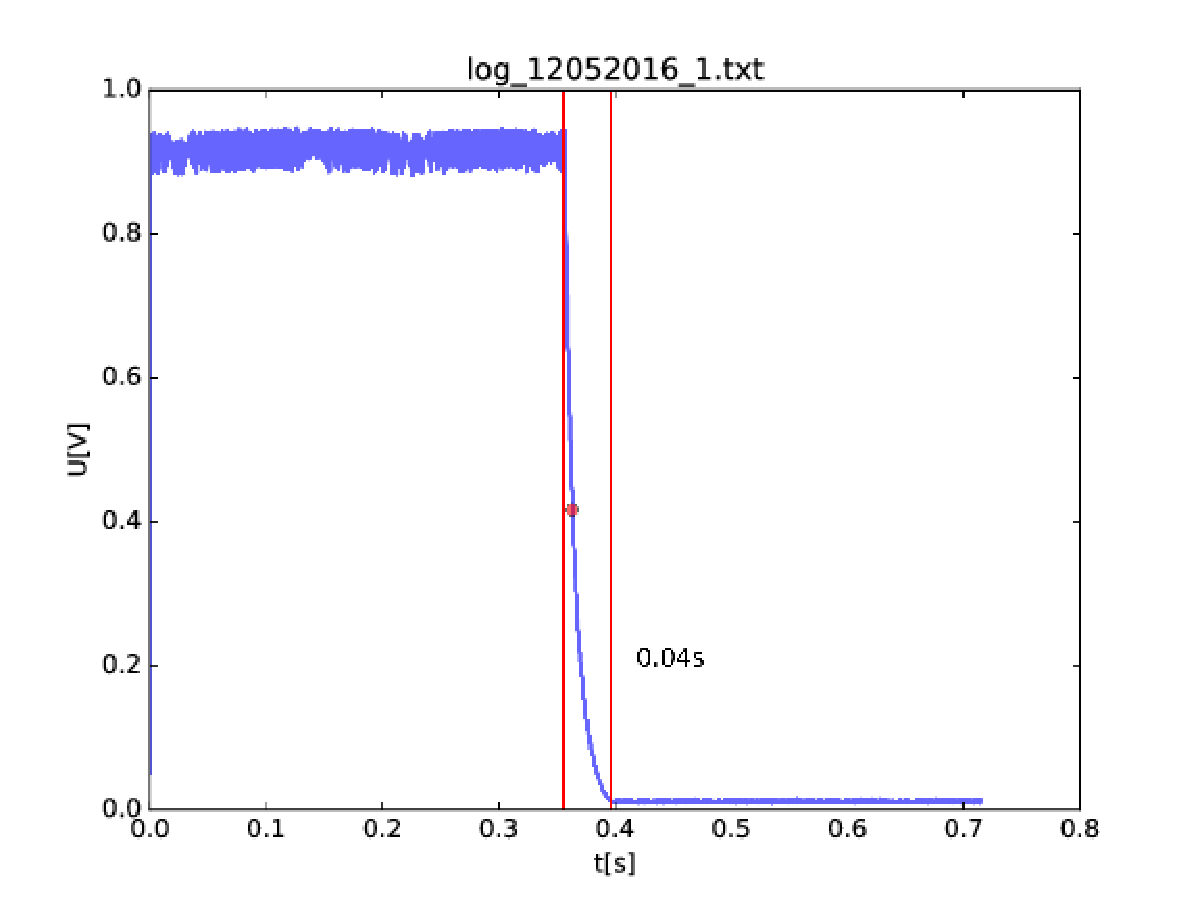
\includegraphics[width=0.8\textwidth]{images/switch_cap.pdf} 
		\caption[The scatter plot shows the measured voltage with a resistance of 0]{The scatter plot shows the measured voltage with a resistance of 0. At the first red line, a switch discontinuous the connection, making the resistance infinite. The voltage drops slowly towards zero and reaches the new value after \unit[0.04]{s}, marked by the second red line.}
		\label{fig:swcap}
	\end{center}
\end{figure}

Figure \ref{fig:swnocap} shows the response to the same switching as before, but with the filter capacitor removed. The diode is still in place and removes the negative voltages from the output. Without the capacitor however, the signal oscillates with the same \unit[1666]{Hz} that the Wien bridge oscillator provides. Because the sample rate of the ADC is not as fast as the oscillation, it measures at random moments on the sine wave, resulting in an output that moves between zero and the maximum amplitude. The red line again marks the moment of the switch and it can be clearly seen that the response delay has disappeared. The oscillating behavior that was electrically filtered before, is now visible and has to be addressed in the data analysis which will be described later in the Section \ref{val} Validation.

\begin{figure}[H]
	\begin{center}
		% This file was created by matplotlib2tikz v0.5.10.
\begin{tikzpicture}

\begin{axis}[
xlabel={Time, s},
ylabel={Voltage, V},
xmin=-0.1, xmax=0.8,
ymin=0, ymax=1,
axis on top,
xtick={-0.1,0,0.1,0.2,0.3,0.4,0.5,0.6,0.7,0.8},
xticklabels={−0.1,0.0,0.1,0.2,0.3,0.4,0.5,0.6,0.7,0.8},
ytick={0,0.2,0.4,0.6,0.8,1},
yticklabels={0.0,0.2,0.4,0.6,0.8,1.0}
]
\addplot [draw=blue, fill=blue, opacity=0.5, mark=*, only marks] table {%
0.0 0.00048828125
0.001 0.945068359375
0.001 0.0
0.001 0.945556640625
0.001 0.0
0.002 0.94482421875
0.002 0.0
0.002 0.407470703125
0.002 0.9443359375
0.003 0.0
0.003 0.945068359375
0.003 0.0
0.004 0.945556640625
0.004 0.0
0.004 0.945068359375
0.004 0.0
0.005 0.0
0.005 0.94482421875
0.005 0.0
0.005 0.945068359375
0.006 0.0
0.006 0.944580078125
0.006 0.0
0.007 0.945068359375
0.007 0.428955078125
0.007 0.0
0.007 0.945556640625
0.008 0.0
0.008 0.94287109375
0.008 0.0
0.009 0.945556640625
0.009 0.0
0.009 0.94580078125
0.009 0.0
0.01 0.0
0.01 0.94384765625
0.01 0.0
0.01 0.94482421875
0.011 0.0
0.011 0.944091796875
0.011 0.0
0.012 0.94482421875
0.012 0.0
0.012 0.942626953125
0.012 0.468505859375
0.013 0.0
0.013 0.945068359375
0.013 0.0
0.014 0.945068359375
0.014 0.0
0.014 0.945068359375
0.014 0.0
0.015 0.945068359375
0.015 0.0
0.015 0.945068359375
0.016 0.0
0.016 0.0
0.016 0.892822265625
0.016 0.0
0.017 0.945068359375
0.017 0.0
0.017 0.945556640625
0.018 0.0
0.018 0.945068359375
0.018 0.0
0.018 0.945068359375
0.019 0.0
0.019 0.945068359375
0.019 0.0
0.02 0.944091796875
0.02 0.0
0.02 0.0244140625
0.021 0.9443359375
0.021 0.0
0.021 0.946044921875
0.021 0.0
0.022 0.945068359375
0.022 0.0
0.022 0.945068359375
0.023 0.0
0.023 0.947021484375
0.023 0.0
0.023 0.945068359375
0.024 0.0
0.024 0.94580078125
0.024 0.0
0.025 0.945068359375
0.025 0.0
0.025 0.945556640625
0.026 0.0
0.026 0.94482421875
0.026 0.0
0.026 0.945068359375
0.027 0.0
0.027 0.945068359375
0.027 0.0
0.028 0.945068359375
0.028 0.0
0.028 0.945068359375
0.029 0.0
0.029 0.944580078125
0.029 0.0
0.03 0.944091796875
0.03 0.0
0.03 0.945068359375
0.03 0.0
0.031 0.128662109375
0.031 0.0
0.031 0.939697265625
0.032 0.0
0.032 0.946044921875
0.032 0.0
0.033 0.89306640625
0.033 0.0
0.033 0.945068359375
0.034 0.0
0.034 0.945068359375
0.034 0.0
0.035 0.945068359375
0.035 0.0
0.035 0.946044921875
0.035 0.0
0.036 0.945068359375
0.036 0.0
0.036 0.946044921875
0.037 0.0
0.037 0.945068359375
0.037 0.0
0.038 0.945068359375
0.038 0.0
0.038 0.94580078125
0.039 0.0
0.039 0.9462890625
0.039 0.0
0.04 0.945556640625
0.04 0.0
0.04 0.945068359375
0.041 0.0
0.041 0.9453125
0.041 0.0
0.042 0.946044921875
0.042 0.0
0.042 0.945068359375
0.042 0.0
0.043 0.94580078125
0.043 0.0
0.043 0.945068359375
0.044 0.0
0.044 0.946044921875
0.044 0.0
0.045 0.946044921875
0.045 0.0
0.045 0.593505859375
0.046 0.0
0.046 0.0
0.046 0.945556640625
0.047 0.0
0.047 0.945068359375
0.047 0.0
0.048 0.945556640625
0.048 0.0
0.048 0.945556640625
0.049 0.0
0.049 0.945068359375
0.049 0.0
0.05 0.945068359375
0.05 0.0
0.05 0.94580078125
0.051 0.0
0.051 0.944580078125
0.051 0.0
0.052 0.599365234375
0.052 0.945068359375
0.052 0.0
0.053 0.945068359375
0.053 0.0
0.053 0.946044921875
0.054 0.0
0.054 0.945068359375
0.054 0.0
0.055 0.94580078125
0.055 0.0
0.055 0.9462890625
0.056 0.0
0.056 0.94677734375
0.056 0.0
0.057 0.187255859375
0.057 0.945068359375
0.057 0.0
0.058 0.945068359375
0.058 0.0
0.058 0.945068359375
0.059 0.0
0.059 0.945068359375
0.059 0.0
0.06 0.94580078125
0.06 0.0
0.06 0.831298828125
0.061 0.0380859375
0.061 0.0
0.061 0.945068359375
0.062 0.0
0.062 0.945556640625
0.062 0.0
0.063 0.946044921875
0.063 0.0
0.063 0.94580078125
0.064 0.0
0.064 0.0
0.064 0.942626953125
0.065 0.0
0.065 0.945068359375
0.065 0.0
0.066 0.9462890625
0.066 0.0
0.066 0.946044921875
0.067 0.0
0.067 0.913330078125
0.067 0.0498046875
0.068 0.0
0.068 0.945068359375
0.068 0.0
0.069 0.945068359375
0.069 0.0
0.07 0.945068359375
0.07 0.0
0.07 0.946044921875
0.071 0.0
0.071 0.0
0.071 0.944580078125
0.072 0.0
0.072 0.945556640625
0.072 0.0
0.073 0.94580078125
0.073 0.0
0.073 0.9462890625
0.074 0.027099609375
0.074 0.0
0.074 0.945556640625
0.075 0.0
0.075 0.946044921875
0.075 0.0
0.076 0.945068359375
0.076 0.0
0.076 0.280517578125
0.077 0.945068359375
0.077 0.0
0.078 0.945068359375
0.078 0.0
0.078 0.945556640625
0.079 0.0
0.079 0.236572265625
0.079 0.945068359375
0.08 0.0
0.08 0.945068359375
0.08 0.0
0.081 0.946044921875
0.081 0.0
0.081 0.495849609375
0.082 0.94677734375
0.082 0.0
0.083 0.94580078125
0.083 0.0
0.083 0.94580078125
0.084 0.0
0.084 0.0
0.084 0.945068359375
0.085 0.0
0.085 0.945556640625
0.085 0.0
0.086 0.94580078125
0.086 0.299560546875
0.086 0.0
0.087 0.945068359375
0.087 0.0
0.088 0.946044921875
0.088 0.0
0.088 0.12060546875
0.089 0.945068359375
0.089 0.0
0.089 0.945068359375
0.09 0.0
0.09 0.945068359375
0.09 0.059326171875
0.091 0.0
0.091 0.945068359375
0.092 0.0
0.092 0.9462890625
0.092 0.0
0.093 0.0
0.093 0.945068359375
0.093 0.0
0.094 0.945068359375
0.094 0.0
0.094 0.946044921875
0.095 0.94482421875
0.095 0.0
0.096 0.945068359375
0.096 0.0
0.096 0.945068359375
0.097 0.025390625
0.097 0.0
0.097 0.945556640625
0.098 0.0
0.098 0.945068359375
0.099 0.0
0.099 0.0
0.099 0.945068359375
0.1 0.0
0.1 0.945556640625
0.1 0.0
0.101 0.0
0.101 0.945068359375
0.101 0.0
0.102 0.945068359375
0.102 0.0
0.103 0.0
0.103 0.94580078125
0.103 0.0
0.104 0.945068359375
0.104 0.0
0.104 0.0
0.105 0.945068359375
0.105 0.0
0.106 0.945068359375
0.106 0.0
0.106 0.0
0.107 0.945068359375
0.107 0.0
0.107 0.945556640625
0.108 0.046142578125
0.108 0.0
0.109 0.945068359375
0.109 0.0
0.109 0.945068359375
0.11 0.663818359375
0.11 0.0
0.111 0.946044921875
0.111 0.0
0.111 0.510009765625
0.112 0.945068359375
0.112 0.0
0.112 0.946044921875
0.113 0.0
0.113 0.0
0.114 0.945068359375
0.114 0.0
0.114 0.945068359375
0.115 0.033447265625
0.115 0.0
0.115 0.945068359375
0.116 0.0
0.116 0.6083984375
0.117 0.945068359375
0.117 0.0
0.117 0.945068359375
0.118 0.0
0.118 0.0
0.119 0.945068359375
0.119 0.0
0.119 0.945068359375
0.12 0.945068359375
0.12 0.0
0.12 0.9462890625
0.121 0.0
0.121 0.0
0.122 0.945068359375
0.122 0.0
0.122 0.945068359375
0.123 0.94482421875
0.123 0.0
0.124 0.945068359375
0.124 0.0
0.124 0.0
0.125 0.943359375
0.125 0.0
0.126 0.945068359375
0.126 0.945068359375
0.126 0.0
0.127 0.945068359375
0.127 0.0
0.128 0.0
0.128 0.945068359375
0.128 0.0
0.129 0.471923828125
0.129 0.94580078125
0.13 0.0
0.13 0.946044921875
0.13 0.946044921875
0.131 0.0
0.131 0.945068359375
0.131 0.0
0.132 0.0
0.132 0.945068359375
0.133 0.0
0.133 0.0
0.133 0.945556640625
0.134 0.0
0.134 0.945068359375
0.135 0.945068359375
0.135 0.0
0.135 0.945068359375
0.136 0.944580078125
0.136 0.0
0.137 0.945068359375
0.137 0.0
0.137 0.0
0.138 0.945068359375
0.138 0.0
0.139 0.0
0.139 0.94580078125
0.139 0.0
0.14 0.0
0.14 0.945068359375
0.141 0.0
0.141 0.945068359375
0.141 0.945068359375
0.142 0.0
0.142 0.945068359375
0.143 0.076904296875
0.143 0.0
0.144 0.945556640625
0.144 0.0
0.144 0.0
0.145 0.9453125
0.145 0.0
0.146 0.0
0.146 0.945068359375
0.146 0.0
0.147 0.0
0.147 0.945068359375
0.148 0.0
0.148 0.0
0.148 0.945068359375
0.149 0.0
0.149 0.626953125
0.15 0.945068359375
0.15 0.0
0.15 0.946044921875
0.151 0.945068359375
0.151 0.0
0.152 0.945068359375
0.152 0.945068359375
0.153 0.0
0.153 0.945068359375
0.153 0.945068359375
0.154 0.0
0.154 0.945068359375
0.155 0.945556640625
0.155 0.0
0.155 0.945068359375
0.156 0.9443359375
0.156 0.0
0.157 0.945068359375
0.157 0.945068359375
0.158 0.0
0.158 0.34423828125
0.158 0.94580078125
0.159 0.0
0.159 0.310546875
0.16 0.945068359375
0.16 0.0
0.16 0.0
0.161 0.945556640625
0.161 0.0
0.162 0.0
0.162 0.945556640625
0.163 0.0
0.163 0.0
0.163 0.945068359375
0.164 0.0
0.164 0.0
0.165 0.945068359375
0.165 0.0
0.165 0.0
0.166 0.944580078125
0.166 0.0
0.167 0.0
0.167 0.94482421875
0.168 0.0
0.168 0.0
0.168 0.945068359375
0.169 0.944091796875
0.169 0.0
0.17 0.947021484375
0.17 0.945068359375
0.171 0.0
0.171 0.946044921875
0.171 0.944580078125
0.172 0.0
0.172 0.083740234375
0.173 0.945068359375
0.173 0.0
0.174 0.0
0.174 0.945068359375
0.174 0.0
0.175 0.0
0.175 0.945068359375
0.176 0.0
0.176 0.0
0.176 0.944580078125
0.177 0.945556640625
0.177 0.0
0.178 0.7431640625
0.178 0.945068359375
0.179 0.0
0.179 0.0
0.18 0.945068359375
0.18 0.0
0.18 0.0
0.181 0.945068359375
0.181 0.0
0.182 0.0
0.182 0.945068359375
0.183 0.87353515625
0.183 0.0
0.183 0.945068359375
0.184 0.944580078125
0.184 0.0
0.185 0.0
0.185 0.945068359375
0.186 0.0
0.186 0.0
0.186 0.945556640625
0.187 0.945068359375
0.187 0.0
0.188 0.0
0.188 0.945068359375
0.189 0.0
0.189 0.0
0.19 0.945556640625
0.19 0.044677734375
0.19 0.0
0.191 0.945556640625
0.191 0.945068359375
0.192 0.0
0.192 0.0
0.193 0.945068359375
0.193 0.0
0.193 0.0
0.194 0.945068359375
0.194 0.945068359375
0.195 0.0
0.195 0.0
0.196 0.9453125
0.196 0.0
0.197 0.0
0.197 0.945068359375
0.197 0.945068359375
0.198 0.0
0.198 0.0
0.199 0.945068359375
0.199 0.0
0.2 0.0
0.2 0.945068359375
0.201 0.945068359375
0.201 0.0
0.201 0.0
0.202 0.945068359375
0.202 0.0
0.203 0.0
0.203 0.945068359375
0.204 0.944580078125
0.204 0.0
0.205 0.0
0.205 0.945068359375
0.206 0.075927734375
0.206 0.0
0.206 0.705810546875
0.207 0.945068359375
0.207 0.0
0.208 0.0
0.208 0.945068359375
0.209 0.94384765625
0.209 0.0
0.21 0.0
0.21 0.945068359375
0.211 0.882568359375
0.211 0.0
0.211 0.097412109375
0.212 0.945068359375
0.212 0.0
0.213 0.0
0.213 0.944580078125
0.214 0.944580078125
0.214 0.0
0.215 0.0
0.215 0.945068359375
0.216 0.945068359375
0.216 0.0
0.216 0.0
0.217 0.945068359375
0.217 0.945068359375
0.218 0.0
0.218 0.0
0.219 0.945068359375
0.219 0.072509765625
0.22 0.0
0.22 0.945068359375
0.221 0.9453125
0.221 0.0
0.221 0.0
0.222 0.945556640625
0.222 0.945068359375
0.223 0.0
0.223 0.0
0.224 0.94580078125
0.224 0.945068359375
0.225 0.0
0.225 0.0
0.226 0.9443359375
0.226 0.945068359375
0.227 0.0
0.227 0.0
0.227 0.945068359375
0.228 0.945068359375
0.228 0.0
0.229 0.0
0.229 0.945068359375
0.23 0.945068359375
0.23 0.0
0.231 0.0
0.231 0.945556640625
0.232 0.943359375
0.232 0.0
0.233 0.0
0.233 0.945556640625
0.234 0.945068359375
0.234 0.0
0.234 0.0
0.235 0.94482421875
0.235 0.945068359375
0.236 0.0
0.236 0.0
0.237 0.945068359375
0.237 0.945068359375
0.238 0.0
0.238 0.0
0.239 0.752685546875
0.239 0.945068359375
0.24 0.045166015625
0.24 0.0
0.241 0.0
0.241 0.945068359375
0.242 0.21044921875
0.242 0.0
0.243 0.0
0.243 0.945068359375
0.243 0.945068359375
0.244 0.0
0.244 0.0
0.245 0.944580078125
0.245 0.944091796875
0.246 0.0
0.246 0.0
0.247 0.898193359375
0.247 0.945068359375
0.248 0.276611328125
0.248 0.0
0.249 0.0
0.249 0.945556640625
0.25 0.945068359375
0.25 0.0
0.251 0.0
0.251 0.945068359375
0.252 0.94482421875
0.252 0.0
0.253 0.0
0.253 0.348876953125
0.254 0.945068359375
0.254 0.94482421875
0.255 0.0
0.255 0.0
0.255 0.944580078125
0.256 0.944091796875
0.256 0.0
0.257 0.0
0.257 0.328857421875
0.258 0.94482421875
0.258 0.945068359375
0.259 0.0
0.259 0.0
0.26 0.9453125
0.26 0.945068359375
0.261 0.641845703125
0.261 0.0
0.262 0.0
0.262 0.945068359375
0.263 0.944091796875
0.263 0.0
0.264 0.0
0.264 0.20458984375
0.265 0.945068359375
0.265 0.9453125
0.266 0.0
0.266 0.0
0.267 0.83203125
0.267 0.945068359375
0.268 0.945068359375
0.268 0.0
0.269 0.0
0.269 0.945068359375
0.27 0.945068359375
0.27 0.0
0.271 0.0
0.271 0.0
0.272 0.944580078125
0.272 0.945068359375
0.273 0.0
0.273 0.0
0.274 0.0
0.274 0.945068359375
0.275 0.943603515625
0.275 0.0
0.276 0.0
0.276 0.0
0.277 0.944580078125
0.277 0.944580078125
0.278 0.0
0.278 0.0
0.279 0.627197265625
0.279 0.945068359375
0.28 0.947265625
0.28 0.0
0.281 0.0
0.281 0.92822265625
0.282 0.945068359375
0.282 0.945068359375
0.283 0.0
0.283 0.0
0.284 0.945068359375
0.284 0.9453125
0.285 0.945068359375
0.285 0.0
0.286 0.0
0.286 0.732177734375
0.287 0.945068359375
0.287 0.945068359375
0.288 0.0
0.288 0.0
0.289 0.747802734375
0.289 0.944580078125
0.29 0.945068359375
0.29 0.0
0.291 0.0
0.291 0.0
0.292 0.945068359375
0.292 0.94482421875
0.293 0.0
0.293 0.0
0.294 0.0
0.294 0.945068359375
0.295 0.945068359375
0.295 0.0
0.296 0.0
0.296 0.0
0.297 0.945068359375
0.297 0.945068359375
0.298 0.0
0.298 0.0
0.299 0.0
0.299 0.945068359375
0.3 0.945068359375
0.3 0.0
0.301 0.0
0.301 0.0
0.302 0.945068359375
0.302 0.945068359375
0.303 0.051025390625
0.303 0.0
0.304 0.0
0.304 0.945068359375
0.305 0.94482421875
0.305 0.945068359375
0.306 0.0
0.306 0.0
0.307 0.0
0.307 0.945068359375
0.308 0.945068359375
0.308 0.9453125
0.309 0.0
0.309 0.0
0.31 0.0
0.31 0.94482421875
0.311 0.945068359375
0.311 0.9453125
0.312 0.0
0.312 0.0
0.313 0.0
0.313 0.945068359375
0.314 0.945068359375
0.314 0.945068359375
0.315 0.0
0.315 0.0
0.316 0.0
0.316 0.945068359375
0.317 0.945556640625
0.318 0.945068359375
0.318 0.0
0.319 0.0
0.319 0.0
0.32 0.0
0.322 0.945068359375
0.322 0.034423828125
0.323 0.0
0.323 0.9453125
0.323 0.0
0.323 0.945068359375
0.324 0.0
0.324 0.945068359375
0.324 0.0
0.325 0.03564453125
0.325 0.69140625
0.325 0.0
0.325 0.945556640625
0.326 0.0
0.326 0.945556640625
0.326 0.0
0.326 0.94482421875
0.327 0.0
0.327 0.02783203125
0.327 0.945068359375
0.328 0.0
0.328 0.944580078125
0.328 0.0
0.328 0.9453125
0.329 0.0
0.329 0.94482421875
0.329 0.0
0.33 0.599609375
0.33 0.15185546875
0.33 0.0
0.33 0.94580078125
0.331 0.0
0.331 0.945556640625
0.331 0.0
0.332 0.944580078125
0.332 0.0
0.332 0.9453125
0.332 0.0
0.333 0.042236328125
0.333 0.121337890625
0.333 0.0
0.333 0.945068359375
0.334 0.0
0.334 0.945556640625
0.334 0.0
0.335 0.945068359375
0.335 0.0
0.335 0.945068359375
0.335 0.0
0.336 0.853759765625
0.336 0.0
0.336 0.0
0.337 0.945068359375
0.337 0.0
0.337 0.945068359375
0.337 0.0
0.338 0.944091796875
0.338 0.0
0.338 0.94580078125
0.339 0.0
0.339 0.945068359375
0.339 0.0
0.34 0.945068359375
0.34 0.0
0.34 0.566650390625
0.34 0.46875
0.341 0.0
0.341 0.947021484375
0.341 0.0
0.342 0.946044921875
0.342 0.0
0.342 0.945556640625
0.342 0.0
0.343 0.947021484375
0.343 0.0
0.343 0.945068359375
0.344 0.0
0.344 0.945556640625
0.344 0.0
0.345 0.945068359375
0.345 0.0
0.345 0.945068359375
0.345 0.0
0.346 0.945068359375
0.346 0.0
0.346 0.060302734375
0.347 0.55419921875
0.347 0.066650390625
0.347 0.53076171875
0.348 0.0
0.348 0.679443359375
0.348 0.0
0.348 0.946044921875
0.349 0.0
0.349 0.945068359375
0.349 0.0
0.35 0.945068359375
0.35 0.0
0.35 0.945556640625
0.351 0.0
0.351 0.945556640625
0.351 0.0
0.351 0.945556640625
0.352 0.0
0.352 0.94580078125
0.352 0.0
0.353 0.946044921875
0.353 0.0
0.353 0.945068359375
0.354 0.0
0.354 0.945068359375
0.354 0.0
0.355 0.945068359375
0.355 0.0
0.355 0.94580078125
0.355 0.0
0.356 0.945068359375
0.356 0.0
0.356 0.946044921875
0.357 0.0
0.357 0.945068359375
0.357 0.0
0.358 0.945556640625
0.358 0.0
0.358 0.94580078125
0.359 0.0
0.359 0.94677734375
0.359 0.0
0.36 0.946044921875
0.36 0.0
0.36 0.946044921875
0.361 0.0
0.361 0.945068359375
0.361 0.0
0.361 0.945068359375
0.362 0.0
0.362 0.637451171875
0.362 0.0
0.363 0.0
0.363 0.051025390625
0.363 0.0
0.364 0.05078125
0.364 0.0
0.364 0.943603515625
0.365 0.0
0.365 0.946044921875
0.365 0.0
0.366 0.946044921875
0.366 0.0
0.366 0.946044921875
0.367 0.0
0.367 0.946044921875
0.367 0.0
0.368 0.945068359375
0.368 0.0
0.368 0.946044921875
0.369 0.0
0.369 0.946533203125
0.369 0.0
0.37 0.946044921875
0.37 0.0
0.37 0.94580078125
0.371 0.0
0.371 0.0
0.371 0.20703125
0.371 0.0
0.372 0.945068359375
0.372 0.0
0.372 0.9462890625
0.373 0.0
0.373 0.945068359375
0.373 0.0
0.374 0.945068359375
0.374 0.0
0.374 0.945556640625
0.375 0.0
0.375 0.945068359375
0.375 0.0
0.376 0.542724609375
0.376 0.038330078125
0.376 0.0
0.377 0.945068359375
0.377 0.0
0.377 0.945068359375
0.378 0.0
0.378 0.946044921875
0.378 0.0
0.379 0.945556640625
0.379 0.0
0.379 0.946044921875
0.38 0.0
0.38 0.893310546875
0.38 0.0
0.381 0.0
0.381 0.945068359375
0.381 0.0
0.382 0.945556640625
0.382 0.0
0.383 0.01416015625
0.383 0.0
0.384 0.014404296875
0.384 0.0
0.384 0.00390625
0.385 0.00341796875
0.385 0.0
0.385 0.0107421875
0.385 0.0
0.386 0.014404296875
0.386 0.0
0.386 0.007080078125
0.386 0.0
0.387 0.0
0.387 0.00830078125
0.387 0.0
0.387 0.014404296875
0.388 0.0
0.388 0.01318359375
0.388 0.0
0.389 0.0
0.389 0.0029296875
0.389 0.0
0.389 0.011962890625
0.39 0.0
0.39 0.01416015625
0.39 0.0
0.391 0.0078125
0.391 0.0
0.391 0.0
0.391 0.0068359375
0.392 0.0
0.392 0.010498046875
0.392 0.0
0.392 0.01416015625
0.393 0.0
0.393 0.00732421875
0.393 0.0
0.394 0.0
0.394 0.004638671875
0.394 0.0
0.394 0.011962890625
0.395 0.0
0.395 0.013916015625
0.395 0.0
0.395 0.011474609375
0.396 0.0
0.396 0.004150390625
0.396 0.000732421875
0.397 0.0
0.397 0.00634765625
0.397 0.0
0.397 0.0126953125
0.398 0.0
0.398 0.01416015625
0.398 0.0
0.399 0.010009765625
0.399 0.0
0.399 0.00439453125
0.399 0.0
0.4 0.0
0.4 0.005615234375
0.4 0.0
0.401 0.01171875
0.401 0.0
0.401 0.01318359375
0.401 0.0
0.402 0.01416015625
0.402 0.0
0.402 0.009033203125
0.403 0.0
0.403 0.005126953125
0.403 0.0
0.403 0.0
0.404 0.003662109375
0.404 0.0
0.404 0.010009765625
0.405 0.0
0.405 0.01171875
0.405 0.0
0.406 0.01416015625
0.406 0.0
0.406 0.014404296875
0.406 0.0
0.407 0.012451171875
0.407 0.0
0.407 0.005615234375
0.408 0.0
0.408 0.00390625
0.408 0.000244140625
0.408 0.0
0.409 0.003662109375
0.409 0.0
0.409 0.00927734375
0.41 0.0
0.41 0.01025390625
0.41 0.0
0.411 0.01318359375
0.411 0.0
0.411 0.013427734375
0.411 0.0
0.412 0.014404296875
0.412 0.0
0.412 0.013916015625
0.413 0.0
0.413 0.013427734375
0.413 0.0
0.414 0.0068359375
0.414 0.0
0.414 0.006103515625
0.414 0.0
0.415 0.001708984375
0.415 0.0
0.415 0.001220703125
0.416 0.00244140625
0.416 0.0009765625
0.416 0.00244140625
0.417 0.0
0.417 0.00244140625
0.417 0.0
0.417 0.006103515625
0.418 0.0
0.418 0.00732421875
0.418 0.0
0.419 0.01025390625
0.419 0.0
0.419 0.010009765625
0.42 0.0
0.42 0.009521484375
0.42 0.0
0.42 0.011474609375
0.421 0.0
0.421 0.010986328125
0.421 0.0
0.422 0.01123046875
0.422 0.0
0.422 0.011474609375
0.423 0.0
0.423 0.01220703125
0.423 0.0
0.424 0.01318359375
0.424 0.0
0.424 0.012451171875
0.425 0.0
0.425 0.011474609375
0.425 0.0
0.425 0.0126953125
0.426 0.0
0.426 0.01171875
0.426 0.0
0.427 0.010986328125
0.427 0.0
0.427 0.011962890625
0.428 0.0
0.428 0.0107421875
0.428 0.0
0.429 0.011474609375
0.429 0.0
0.429 0.009521484375
0.43 0.0
0.43 0.007080078125
0.43 0.0
0.43 0.0078125
0.431 0.0
0.431 0.005126953125
0.431 0.0
0.432 0.001953125
0.432 0.0
0.432 0.00244140625
0.433 0.001708984375
0.433 0.0
0.433 0.001220703125
0.434 0.000244140625
0.434 0.002197265625
0.434 0.0
0.435 0.001953125
0.435 0.0
0.435 0.005615234375
0.436 0.0
0.436 0.012451171875
0.436 0.0
0.437 0.012939453125
0.437 0.0
0.437 0.01416015625
0.438 0.0
0.438 0.013427734375
0.438 0.0
0.438 0.013427734375
0.439 0.0
0.439 0.01123046875
0.439 0.0
0.44 0.007080078125
0.44 0.0
0.44 0.005615234375
0.441 0.001220703125
0.441 0.0
0.441 0.00244140625
0.442 0.0
0.442 0.007568359375
0.442 0.0
0.443 0.013671875
0.443 0.0
0.443 0.01416015625
0.444 0.0
0.444 0.013671875
0.444 0.0
0.445 0.0107421875
0.445 0.0
0.445 0.009033203125
0.446 0.0
0.446 0.002685546875
0.446 0.000732421875
0.447 0.0
0.447 0.006591796875
0.447 0.0
0.448 0.014404296875
0.448 0.0
0.448 0.013671875
0.449 0.0
0.449 0.009521484375
0.449 0.0
0.45 0.00244140625
0.45 0.001220703125
0.45 0.0
0.451 0.0078125
0.451 0.0
0.451 0.013427734375
0.452 0.0
0.452 0.013916015625
0.452 0.0
0.453 0.0107421875
0.453 0.0
0.453 0.007568359375
0.454 0.0
0.454 0.0
0.455 0.004150390625
0.455 0.0
0.455 0.013671875
0.456 0.0
0.456 0.013427734375
0.456 0.0
0.457 0.01123046875
0.457 0.0
0.457 0.003173828125
0.458 0.001220703125
0.458 0.0
0.458 0.0107421875
0.459 0.0
0.459 0.01416015625
0.459 0.0
0.46 0.013427734375
0.46 0.0
0.46 0.010498046875
0.461 0.0
0.461 0.002685546875
0.461 0.001953125
0.462 0.0
0.462 0.012939453125
0.462 0.0
0.463 0.01416015625
0.463 0.0
0.463 0.01123046875
0.464 0.0
0.464 0.001953125
0.464 0.002685546875
0.465 0.0
0.465 0.013916015625
0.465 0.0
0.466 0.0126953125
0.466 0.0
0.467 0.008544921875
0.467 0.001220703125
0.467 0.0
0.468 0.0078125
0.468 0.0
0.468 0.014404296875
0.469 0.0
0.469 0.01171875
0.469 0.0
0.47 0.002685546875
0.47 0.002685546875
0.47 0.0
0.471 0.013916015625
0.471 0.0
0.471 0.013427734375
0.472 0.0
0.472 0.005126953125
0.473 0.0009765625
0.473 0.0
0.473 0.013671875
0.474 0.0
0.474 0.012451171875
0.474 0.0
0.475 0.003173828125
0.475 0.002685546875
0.475 0.0
0.476 0.01416015625
0.476 0.0
0.476 0.012451171875
0.477 0.0
0.477 0.001708984375
0.478 0.003662109375
0.478 0.0
0.478 0.014404296875
0.479 0.0
0.479 0.010498046875
0.479 0.0
0.48 0.0
0.48 0.007080078125
0.48 0.0
0.481 0.013916015625
0.481 0.0
0.481 0.00830078125
0.482 0.002197265625
0.482 0.0
0.483 0.013671875
0.483 0.0
0.483 0.01123046875
0.484 0.0
0.484 0.0
0.484 0.007568359375
0.485 0.0
0.485 0.013427734375
0.485 0.0
0.486 0.002197265625
0.486 0.004638671875
0.487 0.0
0.487 0.0146484375
0.487 0.0
0.488 0.00732421875
0.488 0.0
0.488 0.0
0.489 0.014404296875
0.489 0.0
0.49 0.011474609375
0.49 0.0
0.49 0.0
0.491 0.013916015625
0.491 0.0
0.491 0.01220703125
0.492 0.0
0.492 0.0
0.492 0.0087890625
0.493 0.0
0.493 0.012451171875
0.494 0.0
0.494 0.0
0.494 0.00830078125
0.495 0.0
0.495 0.012451171875
0.495 0.0
0.496 0.0
0.496 0.012451171875
0.497 0.0
0.497 0.01123046875
0.497 0.0
0.498 0.0
0.498 0.013916015625
0.498 0.0
0.499 0.00927734375
0.499 0.0
0.5 0.0
0.5 0.013916015625
0.5 0.0
0.501 0.008544921875
0.501 0.0
0.501 0.0
0.502 0.014404296875
0.502 0.0
0.503 0.004638671875
0.503 0.003662109375
0.503 0.0
0.504 0.013427734375
0.504 0.0
0.505 0.00244140625
0.505 0.0126953125
0.505 0.0
0.506 0.010009765625
0.506 0.0
0.506 0.0
0.507 0.014404296875
0.507 0.0
0.508 0.00732421875
0.508 0.0029296875
0.508 0.0
0.509 0.013427734375
0.509 0.0
0.509 0.001708984375
0.51 0.01318359375
0.51 0.0
0.511 0.0087890625
0.511 0.000732421875
0.511 0.0
0.512 0.013671875
0.512 0.0
0.513 0.0
0.513 0.0126953125
0.513 0.0
0.514 0.008544921875
0.514 0.00146484375
0.515 0.0
0.515 0.01416015625
0.515 0.0
0.516 0.000244140625
0.516 0.009033203125
0.516 0.0
0.517 0.009033203125
0.517 0.00048828125
0.518 0.0
0.518 0.013671875
0.518 0.0
0.519 0.0
0.519 0.013671875
0.52 0.0
0.52 0.005126953125
0.52 0.005126953125
0.521 0.0
0.521 0.01123046875
0.522 0.002197265625
0.522 0.0
0.522 0.013916015625
0.523 0.0
0.523 0.0
0.524 0.014404296875
0.524 0.0
0.524 0.005126953125
0.525 0.0107421875
0.525 0.0
0.526 0.008544921875
0.526 0.0029296875
0.526 0.0
0.527 0.012451171875
0.527 0.0
0.528 0.0
0.528 0.013916015625
0.528 0.0
0.529 0.0
0.529 0.013916015625
0.53 0.0
0.53 0.003662109375
0.53 0.007080078125
0.531 0.0
0.531 0.008544921875
0.532 0.00634765625
0.532 0.0
0.532 0.011474609375
0.533 0.002685546875
0.533 0.0
0.534 0.01171875
0.534 0.0
0.534 0.0
0.535 0.013427734375
0.535 0.0
0.536 0.0
0.536 0.01416015625
0.536 0.0
0.537 0.0
0.537 0.013916015625
0.538 0.0
0.538 0.000244140625
0.539 0.01318359375
0.539 0.0
0.539 0.0048828125
0.54 0.01318359375
0.54 0.0
0.541 0.007080078125
0.541 0.00634765625
0.541 0.0
0.542 0.00732421875
0.542 0.0048828125
0.543 0.0
0.543 0.0087890625
0.543 0.00341796875
0.544 0.0
0.544 0.009521484375
0.545 0.006103515625
0.545 0.0
0.545 0.01025390625
0.546 0.0048828125
0.546 0.0
0.547 0.00830078125
0.547 0.004150390625
0.548 0.0
0.548 0.00927734375
0.548 0.003662109375
0.549 0.0
0.549 0.0087890625
0.55 0.007080078125
0.55 0.0
0.55 0.0087890625
0.551 0.007568359375
0.551 0.0
0.552 0.00439453125
0.552 0.008544921875
0.553 0.0
0.553 0.00341796875
0.553 0.012451171875
0.554 0.0
0.554 0.001708984375
0.555 0.013916015625
0.555 0.0
0.556 0.0
0.556 0.013916015625
0.556 0.0
0.557 0.0
0.557 0.01416015625
0.558 0.0
0.558 0.0
0.558 0.01416015625
0.559 0.0
0.559 0.0
0.56 0.012451171875
0.56 0.0
0.561 0.0
0.561 0.010986328125
0.561 0.002197265625
0.562 0.0
0.562 0.008544921875
0.563 0.009521484375
0.563 0.0
0.564 0.000732421875
0.564 0.013671875
0.564 0.0
0.565 0.0
0.565 0.014404296875
0.566 0.0
0.566 0.0
0.567 0.0126953125
0.567 0.0
0.567 0.0
0.568 0.009765625
0.568 0.00439453125
0.569 0.0
0.569 0.0048828125
0.57 0.013916015625
0.57 0.0
0.57 0.0
0.571 0.014404296875
0.571 0.0
0.572 0.0
0.572 0.0126953125
0.573 0.003173828125
0.573 0.0
0.573 0.009033203125
0.574 0.006591796875
0.574 0.0
0.575 0.001220703125
0.575 0.013427734375
0.576 0.0
0.576 0.0
0.577 0.013916015625
0.577 0.0
0.577 0.0
0.578 0.0107421875
0.578 0.00341796875
0.579 0.0
0.579 0.004150390625
0.58 0.01416015625
0.58 0.0
0.58 0.0
0.581 0.01318359375
0.581 0.0
0.582 0.0
0.582 0.00830078125
0.583 0.012939453125
0.583 0.0
0.584 0.0
0.584 0.01416015625
0.584 0.0
0.585 0.0
0.585 0.01025390625
0.586 0.010498046875
0.586 0.0
0.587 0.0
0.587 0.01416015625
0.588 0.0
0.588 0.0
0.588 0.011474609375
0.589 0.007568359375
0.589 0.0
0.59 0.0
0.59 0.014404296875
0.591 0.0
0.591 0.0
0.592 0.00830078125
0.592 0.007568359375
0.592 0.0
0.593 0.0
0.593 0.013916015625
0.594 0.0
0.594 0.0
0.595 0.005615234375
0.595 0.012939453125
0.596 0.0
0.596 0.0
0.596 0.01318359375
0.597 0.002685546875
0.597 0.0
0.598 0.001220703125
0.598 0.014404296875
0.599 0.0
0.599 0.0
0.6 0.0078125
0.6 0.00927734375
0.6 0.0
0.601 0.0
0.601 0.013427734375
0.602 0.00341796875
0.602 0.0
0.603 0.0
0.603 0.014404296875
0.604 0.0
0.604 0.0
0.605 0.00537109375
0.605 0.013916015625
0.606 0.0
0.606 0.0
0.606 0.012451171875
0.607 0.0078125
0.607 0.0
0.608 0.0
0.608 0.013427734375
0.609 0.004638671875
0.611 0.0
0.611 0.010986328125
0.612 0.0
0.612 0.00146484375
0.612 0.00634765625
0.613 0.0
0.613 0.011962890625
0.613 0.0
0.613 0.013916015625
0.614 0.0
0.614 0.004638671875
0.614 0.001953125
0.614 0.0
0.615 0.009765625
0.615 0.0
0.615 0.014404296875
0.616 0.0
0.616 0.013427734375
0.616 0.0
0.616 0.001708984375
0.617 0.005126953125
0.617 0.0
0.617 0.011962890625
0.617 0.0
0.618 0.01416015625
0.618 0.0
0.618 0.007568359375
0.619 0.0
0.619 0.00146484375
0.619 0.00439453125
0.619 0.0
0.62 0.011962890625
0.62 0.0
0.62 0.013671875
0.62 0.0
0.621 0.013427734375
0.621 0.0
0.621 0.00244140625
0.622 0.0029296875
0.622 0.0
0.622 0.010009765625
0.622 0.0
0.623 0.0126953125
0.623 0.0
0.623 0.014404296875
0.624 0.0
0.624 0.012939453125
0.624 0.0
0.624 0.002197265625
0.625 0.0
0.625 0.0
0.625 0.00830078125
0.626 0.0
0.626 0.011474609375
0.626 0.0
0.626 0.01416015625
0.627 0.0
0.627 0.014404296875
0.627 0.0
0.628 0.0078125
0.628 0.0
0.628 0.002685546875
0.628 0.001953125
0.629 0.0
0.629 0.00537109375
0.629 0.0
0.63 0.010986328125
0.63 0.0
0.63 0.0126953125
0.63 0.0
0.631 0.013671875
0.631 0.0
0.631 0.01416015625
0.632 0.0
0.632 0.01318359375
0.632 0.0
0.633 0.005615234375
0.633 0.0
0.633 0.004150390625
0.633 0.0
0.634 0.002685546875
0.634 0.000244140625
0.634 0.0
0.635 0.003662109375
0.635 0.0
0.635 0.009033203125
0.636 0.0
0.636 0.009765625
0.636 0.0
0.636 0.012451171875
0.637 0.0
0.637 0.012939453125
0.637 0.0
0.638 0.013671875
0.638 0.0
0.638 0.01416015625
0.639 0.0
0.639 0.014404296875
0.639 0.0
0.639 0.013916015625
0.64 0.0
0.64 0.013916015625
0.64 0.0
0.641 0.013916015625
0.641 0.0
0.641 0.013427734375
0.642 0.0
0.642 0.01318359375
0.642 0.0
0.643 0.009033203125
0.643 0.0
0.643 0.012939453125
0.643 0.0
0.644 0.013671875
0.644 0.0
0.644 0.0126953125
0.645 0.0
0.645 0.013671875
0.645 0.0
0.646 0.013916015625
0.646 0.0
0.646 0.013427734375
0.647 0.0
0.647 0.01318359375
0.647 0.0
0.647 0.01025390625
0.648 0.0
0.648 0.01318359375
0.648 0.0
0.649 0.01416015625
0.649 0.0
0.649 0.013916015625
0.65 0.0
0.65 0.014404296875
0.65 0.0
0.651 0.01416015625
0.651 0.0
0.651 0.01416015625
0.652 0.0
0.652 0.013671875
0.652 0.0
0.653 0.013671875
0.653 0.0
0.653 0.01318359375
0.653 0.0
0.654 0.01171875
0.654 0.0
0.654 0.01123046875
0.655 0.0
0.655 0.008544921875
0.655 0.0
0.656 0.004150390625
0.656 0.0
0.656 0.00341796875
0.657 0.002197265625
0.657 0.0
0.657 0.002685546875
0.658 0.0
0.658 0.00732421875
0.658 0.0
0.659 0.013671875
0.659 0.0
0.659 0.01416015625
0.66 0.0
0.66 0.01416015625
0.66 0.0
0.661 0.0126953125
0.661 0.0
0.661 0.011962890625
0.662 0.0
0.662 0.0087890625
0.662 0.0
0.663 0.00390625
0.663 0.0
0.663 0.00048828125
0.664 0.004150390625
0.664 0.0
0.664 0.005859375
0.665 0.0
0.665 0.0126953125
0.665 0.0
0.666 0.013916015625
0.666 0.0
0.666 0.014892578125
0.667 0.0
0.667 0.013671875
0.667 0.0
0.668 0.012451171875
0.668 0.0
0.668 0.00732421875
0.669 0.0
0.669 0.0009765625
0.669 0.002197265625
0.67 0.0
0.67 0.00830078125
0.67 0.0
0.671 0.013427734375
0.671 0.0
0.671 0.01416015625
0.672 0.0
0.672 0.012451171875
0.672 0.0
0.673 0.009521484375
0.673 0.0
0.673 0.00341796875
0.674 0.0009765625
0.674 0.0
0.674 0.005859375
0.675 0.0
0.675 0.013427734375
0.675 0.0
0.676 0.01416015625
0.676 0.0
0.676 0.01318359375
0.677 0.0
0.677 0.009765625
0.677 0.0
0.678 0.00537109375
0.678 0.0
0.678 0.0
0.679 0.004638671875
0.679 0.0
0.679 0.013671875
0.68 0.0
0.68 0.013427734375
0.68 0.0
0.681 0.007080078125
0.681 0.0
0.681 0.0009765625
0.682 0.0068359375
0.682 0.0
0.682 0.013671875
0.683 0.0
0.683 0.0126953125
0.683 0.0
0.684 0.005126953125
0.684 0.0
0.684 0.0
0.685 0.012451171875
0.685 0.0
0.685 0.014404296875
0.686 0.0
0.686 0.0107421875
0.687 0.0
0.687 0.0009765625
0.687 0.00390625
0.688 0.0
0.688 0.01416015625
0.688 0.0
0.689 0.01220703125
0.689 0.0
0.689 0.00634765625
0.69 0.0029296875
0.69 0.0
0.69 0.012939453125
0.691 0.0
0.691 0.01318359375
0.691 0.0
0.692 0.004638671875
0.692 0.001220703125
0.693 0.0
0.693 0.01318359375
0.693 0.0
0.694 0.012939453125
0.694 0.0
0.694 0.007080078125
0.695 0.0029296875
0.695 0.0
0.695 0.012939453125
0.696 0.0
0.696 0.01220703125
0.696 0.0
0.697 0.001220703125
0.697 0.00439453125
0.698 0.0
0.698 0.01416015625
0.698 0.0
0.699 0.009033203125
0.699 0.0
0.699 0.0
0.7 0.0126953125
0.7 0.0
0.7 0.013916015625
0.701 0.0
0.701 0.005126953125
0.702 0.001708984375
0.702 0.0
0.702 0.01416015625
0.703 0.0
0.703 0.010498046875
0.703 0.0
0.704 0.0
0.704 0.011962890625
0.704 0.0
0.705 0.012451171875
0.705 0.0
0.706 0.00048828125
0.706 0.006103515625
0.706 0.0
0.707 0.01416015625
0.707 0.0
0.707 0.00732421875
0.708 0.004150390625
0.708 0.0
0.708 0.014404296875
0.709 0.0
0.709 0.009521484375
0.71 0.001708984375
0.71 0.0
0.71 0.013671875
0.711 0.0
0.711 0.009765625
0.711 0.0
0.712 0.0
0.712 0.013916015625
0.713 0.0
0.713 0.010498046875
0.713 0.0
0.714 0.0
0.714 0.013916015625
0.714 0.0
0.715 0.009033203125
0.715 0.0
0.716 0.0
0.716 0.01416015625
0.716 0.0
0.717 0.00732421875
0.717 0.00048828125
0.717 0.0
0.718 0.01416015625
0.718 0.0
0.719 0.00537109375
0.719 0.0029296875
0.719 0.0
0.72 0.013916015625
0.72 0.0
0.72 0.005126953125
0.721 0.007080078125
0.721 0.0
0.722 0.01220703125
0.722 0.0
0.722 0.0
0.723 0.013671875
0.723 0.0
0.723 0.011474609375
0.724 0.0
0.724 0.0
0.725 0.014404296875
0.725 0.0
0.725 0.008056640625
0.726 0.005126953125
0.726 0.0
0.727 0.012939453125
0.727 0.0
0.727 0.000244140625
0.728 0.013916015625
0.728 0.0
0.728 0.010498046875
0.729 0.0
0.729 0.0
0.73 0.014404296875
0.73 0.0
0.73 0.005615234375
0.731 0.007568359375
0.731 0.0
0.732 0.010986328125
0.732 0.0
0.732 0.0
0.733 0.01416015625
0.733 0.0
0.733 0.002685546875
0.734 0.006591796875
0.734 0.0
0.735 0.010986328125
0.735 0.0
0.735 0.0
0.736 0.01416015625
};
\addplot [red, opacity=0.25]
table {%
0.382 0
0.382 1
};
\path [draw=red, fill=red, opacity=0.5] (axis cs:0.382,0.77)
--(axis cs:0.372,0.8)
--(axis cs:0.3815,0.8)
--(axis cs:0.3815,1)
--(axis cs:0.3825,1)
--(axis cs:0.3825,0.8)
--(axis cs:0.392,0.8)
--cycle;

\path [draw=black, fill opacity=0] (axis cs:-0.1,0)
--(axis cs:0.8,0);

\path [draw=black, fill opacity=0] (axis cs:-0.1,1)
--(axis cs:0.8,1);

\path [draw=black, fill opacity=0] (axis cs:0,0)
--(axis cs:0,1);

\path [draw=black, fill opacity=0] (axis cs:1,0)
--(axis cs:1,1);

\end{axis}

\end{tikzpicture}
		%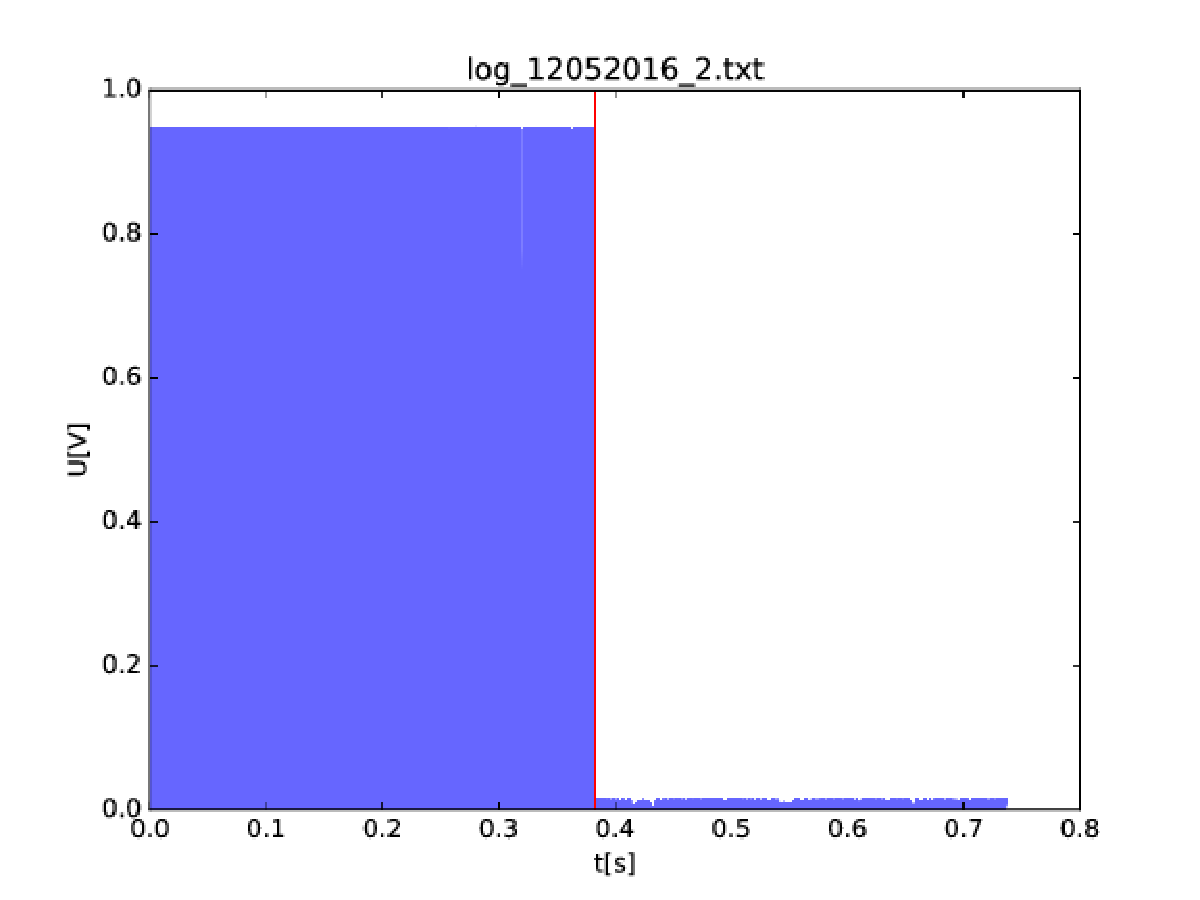
\includegraphics[width=0.8\textwidth]{images/switch_nocap.pdf} 
		\caption[The scatter plot shows the signal oscillating between 0 and the voltage at a resistance of 0]{The scatter plot shows the signal oscillating between 0 and the voltage at a resistance of 0. The red line marks the disconnection. The signal follows without delay.}
		\label{fig:swnocap}
	\end{center}
\end{figure}

\section{Microcontroller} \label{uc}

The microcontroller has to be able to control the functions of the components attached to it. It has to read the data from the MinieC and serve it to the user-interface. They usually are programmed in C or C++, however, in recent years other options emerged. One of those is \textcite{upy}, which is an implementation of the Python 3 programming language designed to run on microcontrollers. As a scripting language, Python is a vastly easier language to work with than C/C++, and helps to speed up the development process. Scripting languages are also often familiar to the targeted users of this device from usage for data processing and visualization. Using MicroPython allows us to design a system where it is more likely that  people using it are able to quickly understand the code, enabling them to improve or adapt it for alternative purposes.
It does however limit our choice of hardware to supported platforms and it requires more powerful and thus more expensive micro-controllers. But as the system only requires one microcontroller to drive a very large amount of sensors, the added cost is relatively small and outweighed by the benefits of the better usability.\\

For prototyping, a development board named "Espruino Pico" was chosen. It is a very small and simple board that provides the electrical boilerplate to use a micro-controller without needing to deal with the lowest level of electronics. It provides a stable power supply and an USB connection to a host PC for programming and exporting the collected data.

\section{Carrier Board}

The carrier board is a simple printed circuit board (PCB) implementing all parts described above. Figure \ref{fig:cb} depicts the assembled board. On the left, the Espruino Pico board can either be soldered directly to the PCB or plugged in using pin header connectors. Above and beyond used pins are replicated on through-holes. This allows an easy connection of measurement equipment to debug the system during development, but can also be used later to connect carrier boards together. Only one would carry a microcontroller and control the other connected boards.

\begin{figure}[H]
	\begin{center}
		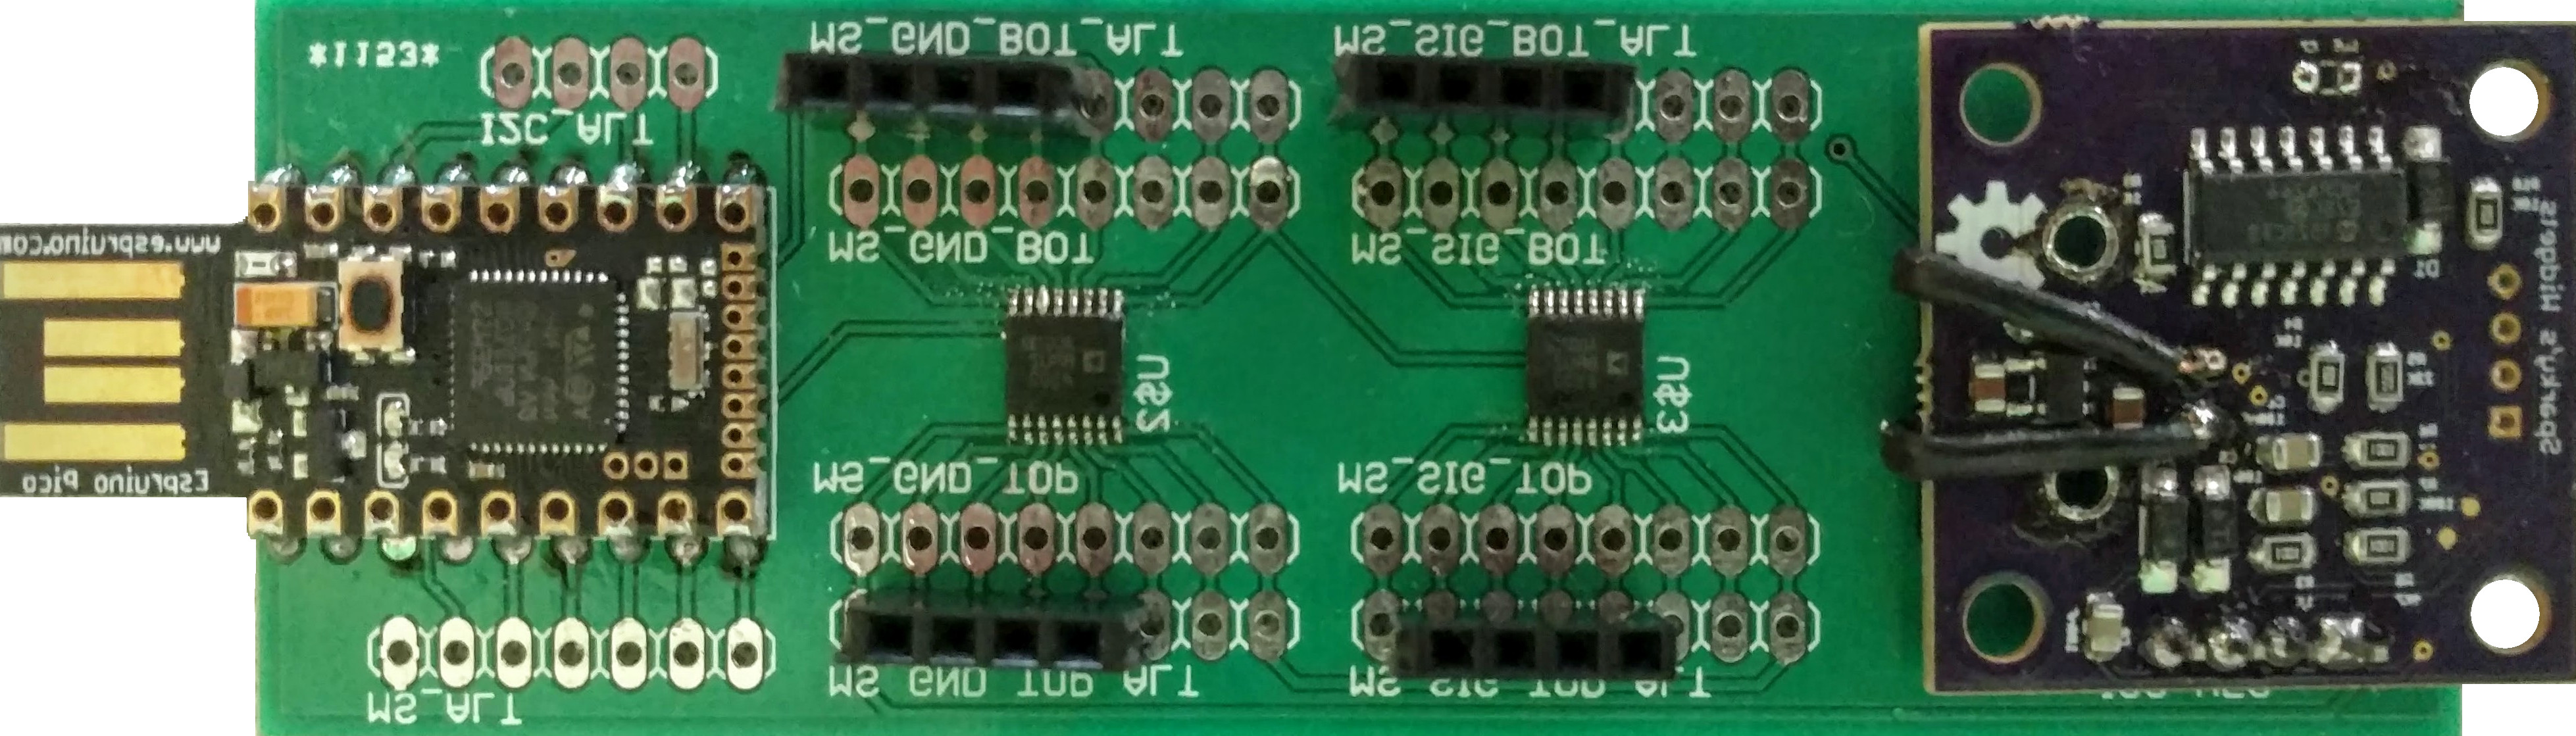
\includegraphics[width=0.8\textwidth]{images/cb.jpg} 
		\caption{The assembled carrier board with all parts directly soldered on}
		\label{fig:cb}
	\end{center}
\end{figure}

Two matrix switches are placed in the middle. They can either be directly soldered on as in this image or they can be soldered to an adapter board that is again mounted to the carrier board with pin header connectors in the inner rows of through-holes.  The outer through-holes are where the connectors for the cables to the sensors are mounted.

The MinieC is located on the right-hand side. It can also be either directly soldered or used with pin header connectors. Additionally, two wires have to be run to the carrier board because of a misalignment of ports due to a design flaw.

The design is tailored to be use as a prototype, meaning that everything is made bigger than necessary, which allows for easier modifications. It is also kept modular, so that each part can be swapped out separately. A later redesign would integrate all boards into one and try to reduce size, which in turn saves money on PCB manufacturing. However, the prototype showed no critical design errors and is fully functional, so the next design step would be only necessary when more boards are needed.

\section{OpenSalinityGUI}

The OpenSalinityGUI is a Graphical User Interface (GUI) designed during this thesis to simplify and aid the usage of the sensor system. It provides the following functions:

\begin{itemize}
	\item Storing all sensor data to a file.
	\item Choosing a file to which the data is stored.
	\item Starting and stopping the data capture.
	\item Visualizing the data.
\end{itemize}

The "Save" button allows to create the file to be written to and offers a default file name containing the date and time of creation, helping to keep the data logs in order. Once a file to save to is chosen, the data capturing can be started by clicking the "Start" button.
The live visualization is a bar graph showing each sensor's current measurement, allowing to monitor the ongoing experiment. In addition to size, the bars are also color coded, shifting from red to blue with increasing salinity. Figure \ref{fig:gui} demonstrates the GUI in use.

The software again is written in Python, using Gtk+ as GUI toolkit and pySerial to communicate with the microcontroller. It was developed and tested on a Linux-based operating system. Furthermore, due to the nature of the used programming language and toolkits, it is cross-platform and can be run on Windows and OSX also.\\

\begin{figure}[H]
	\begin{center}
		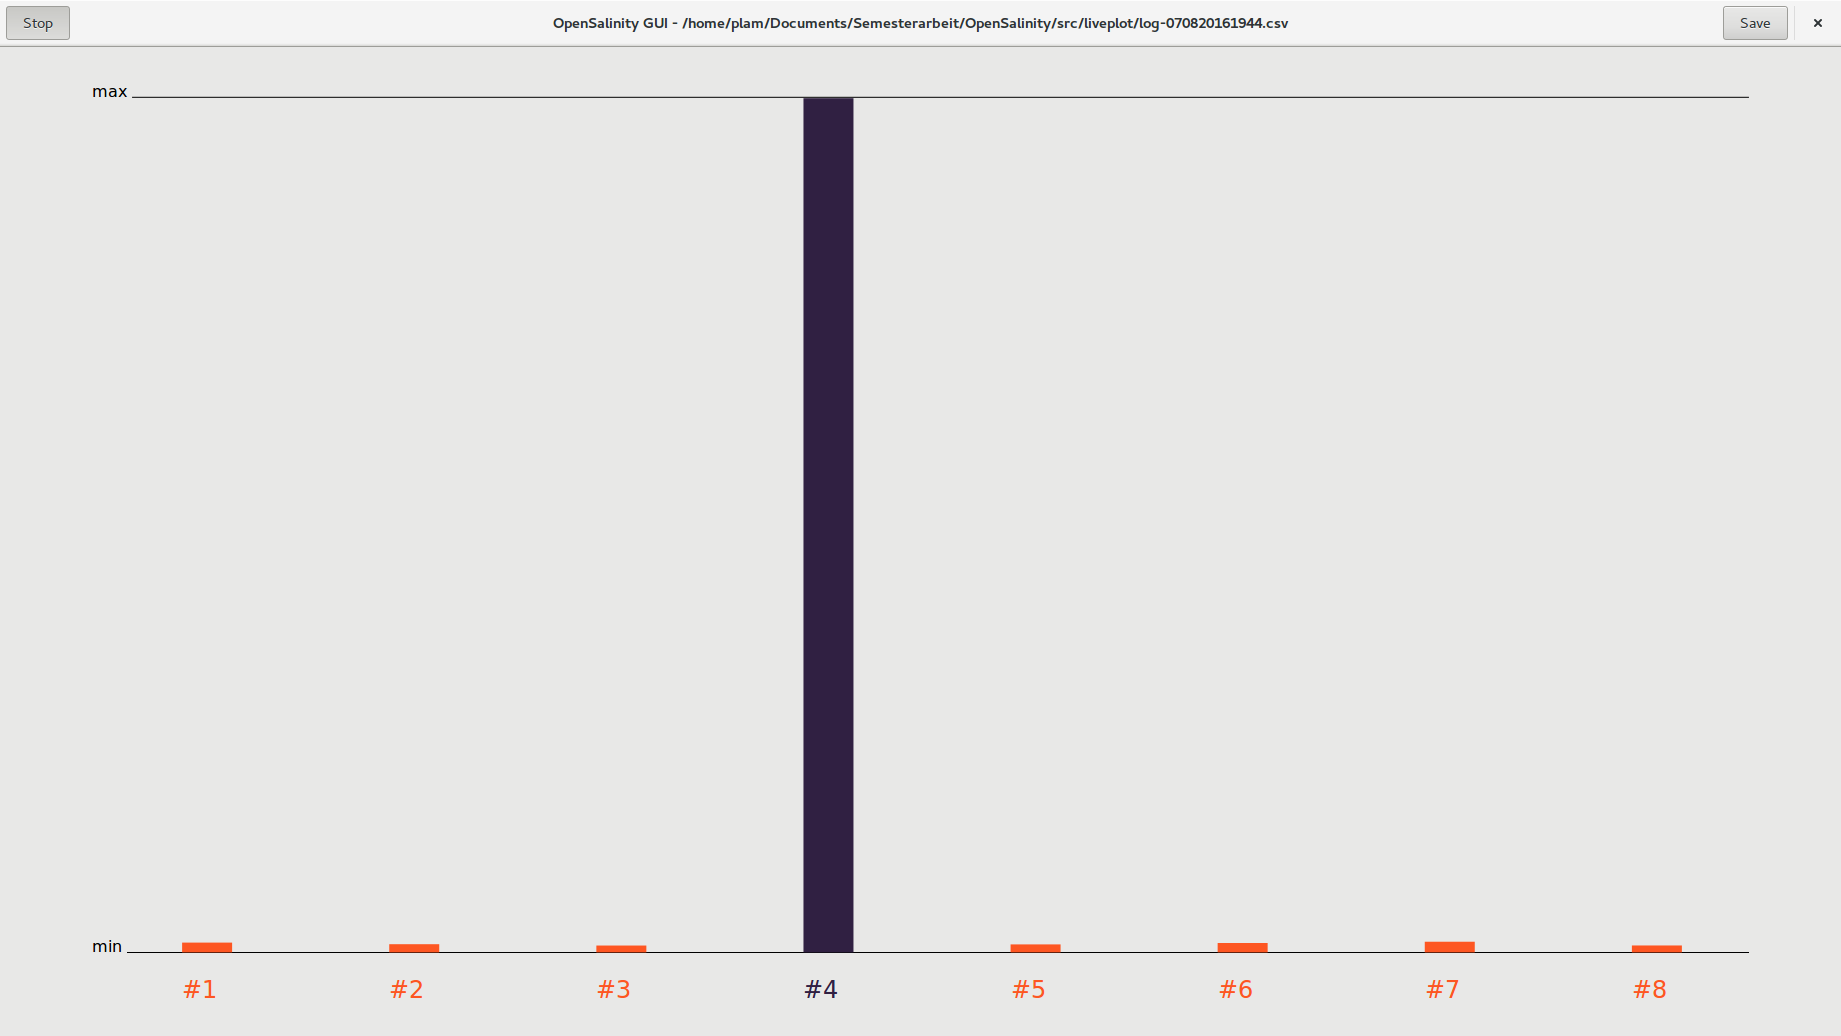
\includegraphics[width=\textwidth]{images/UI.png}
		\caption[OpenSalinityGUI]{OpenSalinityGUI - In this example, sensor $\#4$ measures a resistance of zero (shorted with a wire), all others an infinite resistance (air gap). The "Start/Stop" button is on the top left, the "Save" button on the top right. The path to the chosen file is displayed in the header bar.}
		\label{fig:gui}
	\end{center}
\end{figure}

In addition to or as replacement of the GUI, a set of standard command line interface (CLI) tools can be used. These tools allow for a redundant capturing of the sensor data and for an alternative visualization. Usage of the CLI tools is less intuitive, but they are more robust and faster than the GUI. A detailed manual on how to use those tools as well as the GUI is provided in the Appendix \ref{aman}.

\section{Embedded Software}

The embedded software is the program running on the microcontroller. As already described in Section \ref{uc} Microcontroller, MicroPython is used to implement this program.\\

Figure \ref{fig:flow} shows the flow diagram of the software.
As soon as the system is powered up, it starts listening for the start and stop commands from the OpenSalinityGUI running on the host PC. Communication happens via a serial connection on the USB port. Once a Start command is received, polling of the sensors is started and the data is delivered to the PC, where it is captured and stored.
In order to poll the sensors, the program has to control the switches and the ADC. It first switches both matrix switches to a certain electrode pair and then reads the ADC value for it. Thereafter it switches to the next pair and thus cycles through all connected sensors. Each ADC read is accompanied by a time stamp for the read. Simultaneously the device keeps listening for signals from the GUI in an asynchronous fashion. A stop signal can be received at any time and is executed immediately.\\

The data is sent in a simple format described in the Listing \ref{lst:format}. One line contains timestamps and values for all $n$ connected sensors separated by one whitespace. The line ends with the newline character.

\begin{lstlisting}[caption={The data format contains timestamps and values separated by one whitespace.},label={lst:format}]
<time 1> <value 1> <time 2> <value 2> ... <time n> <value n> \n
<time 1> <value 1> <time 2> <value 2> ... <time n> <value n> \n
...
\end{lstlisting}

\begin{figure}[H]
	\begin{center}
\begin{tikzpicture}[scale=1, rect/.style={minimum width={width("timestamp")+16pt}}]
	%\begin{pgfonlayer}{nodelayer}
		\node [style=scircle, inner sep=6pt, fill=Green!20!White, draw=Green!20!White,align=center, minimum width={width("control")+12pt},] (0) at (0, 16) {power:\\on};
		\node [style=scircle, inner sep=6pt, fill=Green!20!White, draw=Green!20!White, align=center] (1) at (0, 12.5) {control:\\start};
		\node [style=diamond, inner sep=8pt, align=center, fill=Blue!20!White, draw=Blue!20!White] (2) at (0, 9) {while\\i < n};
		\node [style=rect, inner sep=8pt, align=center, fill=Yellow!20!White, draw=Yellow!20!White] (3) at (0, 6) {switch to\\sensor i};
		\node [style=rect, inner sep=8pt, align=center, fill=Yellow!20!White, draw=Yellow!20!White] (4) at (0, 4) {read ADC};
		\node [style=rect, inner sep=8pt, align=center, fill=Yellow!20!White, draw=Yellow!20!White] (5) at (0, 2) {create\\timestamp};
		\node [style=rect, inner sep=8pt, align=center, fill=Blue!20!White, draw=Blue!20!White] (6) at (0, 0) {i++};
		\node [style=rect, inner sep=8pt, align=center, fill=Yellow!20!White, draw=Yellow!20!White] (7) at (4, 9) {send data\\to GUI};
		\node [style=rect, inner sep=8pt, align=center, fill=Blue!20!White, draw=Blue!20!White] (8) at (4, 11) {i = 0};
		
	\node [style=scircle, inner sep=6pt, fill=Red!20!White, draw=Red!20!White,align=center, minimum width={width("control")+12pt},] (100) at (-7, 16) {power:\\off};
	
	\node [style=scircle, inner sep=6pt, fill=Green!20!White, draw=Green!20!White,align=center, minimum width={width("control")+12pt},] (200) at (-4, 16) {power:\\on};
	\node [style=scircle, inner sep=6pt, fill=Red!20!White, draw=Red!20!White, align=center] (201) at (-4, 12.5) {control:\\stop};
	%\end{pgfonlayer}
	
	%\begin{pgfonlayer}{edgelayer}
		\draw [style=arrow, ultra thick] (0) to (1);
		\draw [style=arrow, ultra thick] (200) to (201);
		\draw [style=arrow, ultra thick] (1) to (2);
		\draw [style=arrow, ultra thick] (2) to node[right] {true} (3);
		\draw [style=arrow, ultra thick] (3) to (4);
		\draw [style=arrow, ultra thick] (6) to (-2,0) to (-2,9) to (2);
		\draw [style=arrow, ultra thick] (4) to (5);
		\draw [style=arrow, ultra thick] (5) to (6);
		\draw [style=arrow, ultra thick] (2) to node[below] {false} (7);
		\draw [style=arrow, ultra thick] (7) to (8);
		\draw [style=simple, ultra thick] (8) to (0,11);
		\draw [dashed] (-5.5,17) -- (-5.5,-0.5);
		\draw [dashed] (-2.5,17) -- (-2.5,-0.5);
	%\end{pgfonlayer}
\end{tikzpicture}
		\caption[Embedded Software Flow Diagram]{Embedded Software Flow Diagram - If the power state of the device is "on" and  the control state is "start", data is collected. The control state is set by a signal sent from the GUI and can be changed asynchronously. Data collection is done in a while-loop that runs as long as the iterator i is smaller than the number of sensors n. In the loop, first the matrix switches are set to the i-th sensor, then the ADC is read and afterwards a timestamp is created. When the cycle through all sensors is finished, the data is sent to the GUI. Then the loop is started again. This happens until either the control state switches to "stop" or the power state to "off".}
		\label{fig:flow}
	\end{center}
\end{figure}

\section{Data Conditioning}

Before the data can be analyzed it has to be conditioned to deal with certain peculiarities of the embedded software. This is done in post-processing rather than during the data capturing to minimize overhead and retain high sampling rates.\\

The microcontroller measures time since start-up by counting clock cycles. These are converted to microseconds stored as an integer value. The microcontroller is a 32-bit architecture, nevertheless, the MicroPython implementation uses 2 bits for data type identification, leaving 30 bits for data. This means the counter can cover the range from $-2147483647$ to $2147483647$, resulting in a wrap around after roughly $8.9$ minutes. In the data conditioning phase, these wrapping times are translated to a rolling time since start-up. This is done by scanning for the first time value which is smaller than its predecessor and then adding the value of $2^{30}$ to all following values. This is repeated until all time values are corrected. Figure \ref{fig:wrap} visualizes the algorithm.\\

\begin{figure}[H]
	\begin{center}
\begin{tikzpicture}[scale=1]
    \draw[darrow] (2.5,0) node(xline)[right] {$n$} -|
     (0,2.5) node(yline)[left] {$t$};
     
	\draw (0,0) -- (0.75,1) -- (0.75,-1) -- (2.25,1) -- (2.25,-1) -- (2.5,-0.66);
			
	\draw [style=arrow, bend left=60] (1.5,3.5)to node[above]{first pass} (3.5,3.5);
     
     \draw[darrow] (6,0) node(xline)[right] {$n$} -|
     (3.5,2.5) node(yline)[left] {$t$};
     
	\draw (3.5,0) -- (4.25,1) -- (5.75,3) -- (5.75,1) -- (6,1.33);     
     
	\draw [style=arrow, bend left=60] (6,3.5)to node[above]{second pass} (8,3.5);     
     
     \draw[darrow] (9.5,0) node(xline)[right] {$n$} -|
     (7,2.5) node(yline)[left] {$t$};
     
     \draw (7,0) -- (9.5,3.33);   
     
\end{tikzpicture}
		\caption{Fixing the integer wrap of the time variable}
		\label{fig:wrap}
	\end{center}
\end{figure}

\section{Bill of Materials} \label{BOM}

The bill of materials collects all used components, their price and the source utilized during this project in Table \ref{tab:bom}. Multiple sources are available for all components, except for the MinieC. In case it becomes unavailable, its hardware design files are provided, so they could be manufactured by a different source if need be. The Espruino Pico is produced by a small manufacturer and may also not be available in the future. However, alternatives are plentiful and can be used either with simple jumper cables or by redesigning the carrier board to accommodate the different footprint.

The carrier board and sensor strip are made to order by PCB manufacturers. Generally, any manufacturer will be able to produce the boards with the provided design files, but the size limits and corresponding prices can vary. The costs also strongly depend on lot size. The prices in the table are per piece for a lot of ten carrier boards and 16 sensor strips.

\begin{table}[H]
    \centering

    \caption[Bill of Materials]{Bill of Materials}
    \label{tab:bom}
    \begin{tabular}{llllr}
        	\toprule
        	Nr. & Qt. & Name & Source & Price, \euro{}/pt  \tabularnewline
        	\midrule
		1 & 1 & Espruino Pico & watterott.com & 26.95 \tabularnewline
		2 & 1 & Sparky's Widgets MinieC Interface & sparkyswidgets.com & 21.66 \tabularnewline
		3 & 2 & Analog Devices ADG738 & mouser.de & 3.89 \tabularnewline
		4 & 1 & Carrier Board & dirtypcbs.com & 4.87 \tabularnewline
		5 & 2 & Sensor Strip & leiton.de & 23.53 \tabularnewline
		6 & 1 & USB Extension Cable & amazon.de & 5.49 \tabularnewline
		7 & 1 &  Flat Ribbon Cable 40-pole & amazon.de & 7.99 \tabularnewline
        \bottomrule
    \end{tabular}
\end{table}

\section{List of Software}

Table \ref{tab:sw} lists all software used in this project, including the version numbers. All involved software is Open Source and can be obtained freely. The packages used to analyze and plot the data are provided at the end of the list. Nevertheless, the documented data format should enable the user to replace those with whatever tools he or she is most comfortable with. All software written during this project is provided under the MIT license.

\begin{table}[H]
    \centering

    \caption[List of Software]{List of Software}
    \label{tab:sw}
    \begin{tabular}{lllp{0.25\textwidth}}
        	\toprule
        	Name & Version & Source & Purpose \tabularnewline
        	\midrule
		MicroPython & 1.8.2 & micropython.org & microcontroller firmware \tabularnewline
		Python 3 & 3.5.2 & python.org & GUI and data analysis \tabularnewline
		PyGI 3 & 3.20 & wiki.gnome.org/Projects/PyGObject & GUI toolkit \tabularnewline
		pySerial 3 & 3.0.1 & pythonhosted.org/pyserial & host to microcontroller communication \tabularnewline
		NumPy 3 & 1.11.0 & numpy.org & data analysis \tabularnewline
		SciPy 3 & 0.17.0 & scipy.org & data analysis \tabularnewline
        \bottomrule
    \end{tabular}
\end{table}